\documentclass{article}
\usepackage{polski}
\usepackage[utf8]{inputenc}
\usepackage{indentfirst}  
\usepackage[english]{babel}
\usepackage[left=2.5cm,right=2.5cm,top=2cm,bottom=2cm]{geometry}
\usepackage{graphicx}
\usepackage{listings}
\usepackage{xcolor}
\usepackage{amsmath}
\usepackage{tabularx}
\usepackage{tabulary}
\usepackage{caption}
\captionsetup[table]{name=Tabela}
\overfullrule=1mm
\definecolor{codegreen}{rgb}{0,0.6,0}
\definecolor{codegray}{rgb}{0.5,0.5,0.5}
\definecolor{codepurple}{rgb}{0.58,0,0.82}
\definecolor{backcolour}{rgb}{0.95,0.95,0.92}
\lstdefinestyle{mystyle}{
	backgroundcolor=\color{backcolour},   
	commentstyle=\color{codegreen},
	keywordstyle=\color{magenta},
	numberstyle=\tiny\color{codegray},
	stringstyle=\color{codepurple},
	basicstyle=\ttfamily\footnotesize,
	breakatwhitespace=false,         
	breaklines=true,                 
	captionpos=b,                    
	keepspaces=true,                 
	numbers=left,                    
	numbersep=5pt,                  
	showspaces=false,                
	showstringspaces=false,
	showtabs=false,                  
	tabsize=2
}
\lstset{style=mystyle}
\graphicspath{ {./assets/} }
\parindent=10ex


\begin{document} %---------------------------------------------------------------------------------------------------------------------% 
	
\begin{titlepage}
	\begin{center}
		\vspace{0.5cm}
		
		\Large
		Uniwersytet Gdański\\
		Wydział Matematyki, Fizyki i Informatyki\\
		
		\vspace{2cm}
		
		\textbf{Jakub Lebiedziński}\\
		\vspace{0.75cm}
		Kierunek: Informatyka\\
		Profil: Ogólnoakademicki\\
		Numer albumu: 269096
		
		\vspace*{3cm}
		
		\LARGE
		\textbf{Wykorzystanie cyfrowej analizy obrazu w metodykach pracy z dziećmi w wieku przedszkolnym}   
		
		\begin{flushright}
			\vfill
			
			Praca magisterska napisana\\ pod kierunkiem\\
			dr inż. Arkadiusza Mirakowskiego
		\end{flushright}            
		
		\vspace{2.5cm}
		Gdańsk, 2021    
		
	\end{center}
\end{titlepage}


	
	\linespread{1.3} % interlinia dla dalszej zawartości dokumentu = 1.5
	\large % wielkość czcionki dla dalszej zawartości dokumentu
	
	\newpage
	\renewcommand*\contentsname{Spis treści}
	\tableofcontents
	\newpage
	
	\renewcommand{\figurename}{Rysunek}
	
	\section*{Wstęp}
	
	\par
	Prawdopodobnie czytając te słowa w niedalekiej odległości kilku metrów od czytelnika znajdują się co najmniej trzy urządzenia elektroniczne podłączone do Internetu. Dzieje się tak, ponieważ obecny świat wymaga dostępu do małych komputerków z potężną mocą obliczeniową (porównując oczywiście do urządzeń sprzed kilku dekad), dzięki której nasze życie jest równie proste co skomplikowane. Dlaczego? Nie, nie dlatego, że nie potrafimy kupić elektronicznego biletu z aplikacji. Również nie dlatego, że momentami mamy wrażenie jakoby telefon był mądrzejszy od jego posiadacza i sam mówił mu co ma robić. Możliwości jakie dają nam urządzenia wykorzystujące dzisiejszą technologię przekraczają wszelkie wyobrażenie normalnego człowieka. Potęga mocy obliczeniowej i wielozadaniowości w jaką wyposażona jest niemalże każda maszyna, począwszy od kamery monitoringu, skończywszy na serwerowni wielkiej korporacji OVH zaopatrującą pół Europy w dostęp do sieci WWW, stawia przed nami wyzwanie. Wyzwaniem tym jest umiejętne jej wykorzystanie w celu poprawy i ułatwienia naszego życia jednocześnie balansując między prostotą a skomplikowaniem.
	Celem niniejszej pracy magisterskiej będzie wskazanie na rosnącą rolę technologii cyfrowej w kontekście\linebreak edukacji w ujęciu ogólnym. Moim celem jest udowodnienie, że dzieci w wieku przedszkolnym są w dzisiejszych czasach na tyle zaznajomione z techniką, że są w stanie uczyć się nowych rzeczy z wykorzystaniem ww. technologii. Praca podzielona jest na pięć rozdziałów.
	\par 
	Pierwszy z nich jest wstępem do tematyki ogólnej edukacji dzieci z elementami wykorzystującymi pomoce dydaktyczne. Zwraca szczególną uwagę na postrzeganie świata przez dzieci i doświadczanie go za pomocą zmysłów. Czytając go przemierzamy tysiące lat, od starożytności po czasy nowożytne skupiając się na roli i potrzebie nauki. Poznajemy metody kształcenia, które w swoich czasach uważano za skuteczne, a także podważamy je porównując z dowodami lat późniejszych.
	\par
	W drugim rozdziale niniejszej pracy kładę większy nacisk na edukację w dwudziestym wieku i początek epoki przemysłowej, która niewątpliwie była początkiem rozwoju technologii informatycznej, o której mowa w poniższych rozważaniach.
	\par
	Trzeci rozdział poświęcam czysto technologicznym rozważaniom na tematy cyfrowej analizy i przetwarzania obrazów. Wskazuję wady i zalety niektórych rozwiązań. Rozbijam na czynniki pierwsze prototypy fotografii cyfrowej i analizuje sposób działania analogowych urządzeń do uwieczniania świata na “kawałku taśmy”.
	\par
	Przedostatni rozdział opisuje najświeższe rozwiązania współczesnej techniki wykorzystujące obraz jako kontener z danymi do analizy i implementacji różnego rodzaju algorytmów. Dodatkowo zawiera moje przypuszczenia i przewidywania kierunku, w którym zmierza dzisiejsza technologia w kontekście cyfrowej analizy i przetwarzania obrazów.
	\par
	Piąty i ostateczny rozdział to szczegółowe przedstawienie omawianego celu pracy magisterskiej. Opisuje charakter badań, opis obserwacji oraz wnioski ze szczególnym \linebreak naciskiem na postawioną hipotezę. Na końcu zawiera stwierdzenie potwierdzające lub odrzucające stanowisko w sprawie postawionego przeze mnie celu tej pracy.
	\par
	Całość pracy jest okraszona fotografiami schematów, porównań, fragmentami oprogramowania stworzonego na potrzeby badań oraz bibliografią, na podstawie której zebrałem informacje do napisania poniższej pracy.
	
	\section{Historia edukacji w pojęciu nauczania najmłodszych}
	\subsection{Edukacja kiedyś a edukacja dziś}
	
	\par
	Edukacja jest z nami od zarania dziejów. Już w starożytnej Grecji powstawały pierwsze ‘szkoły’, gdzie słuchacze mogli śledzić wykłady najznamienitszych filozofów ówczesnego świata. Platon, Arystoteles czy Sokrates byli uważani za mistrzów retoryki, etyki czy filozofii. Warto wspomnieć, że nie każdy obywatel antycznego państwa miał obowiązek pobierania nauki. Edukacja była bowiem przywilejem, na który stać było tylko najbogatszych. Dzisiaj jest to nie do pomyślenia. Z czasem jednak edukacja stawała się coraz bardziej dostępna dla niższych warstw społecznych. Dawni nauczyciele wspomagali się w edukowaniu swoich słuchaczy wskaźnikami, elementami natury, mapami, malunkami i tak dalej. Podobnie jest i teraz. Różnicą jest stopień zaawansowania ‘pomagaczy’ i procent ich wykorzystania w szkolnictwie.
	\par
	Nie sposób napisać ile się zmieniło przez tysiące lat, ale jedno jest pewne - jak napisał Marcin Bojarski w swoim felietonie\cite{ref1} “Przekazywanie wiedzy młodszym przez osoby doświadczone jest najpewniej procesem tak starym jak człowiek”. Trudno się nie zgodzić. Od momentu poczęcia, jeszcze zanim ujrzymy świat, w naszym zachowaniu da się dostrzec pewne schematy wyuczone przez te kilka miesięcy etapu płodowego, który trwa między jedenastym, a czterdziestym tygodniem okresu prenatalnego.
	\par
	Nie będę cofał się aż do czasów Adama i Ewy, ale postaram się zacząć od spojrzenia na edukacja w czasach antycznych. Do czasu wynalezienia pisma starsi przekazywali swoje mądrości w sposób werbalny i wymagający zapamiętania dla przyszłych pokoleń. Jakże wielkim wynalazkiem było wynalezienie pisma i zdjęcie obowiązku z człowieka z zapamiętywania wszystkiego co mówił dziadek - niech żyje pismo! Od tego momentu edukacja jako przekazywanie wiedzy nabrała tempa. W starożytnym Egipcie i Mezopotamii wybrańcami, którzy posiedli umiejętność zapisywania i czytania była kasta skrybów, którzy służyli władcy i jego rodzinie. W głównej mierze uczono matematyki, ale też czytania i pisania, co wówczas nie należało do podstawowych umiejętności dorosłego człowieka. Swoistym testamentem tamtych czasów są zachowane, nierzadko w idealnym stanie, hieroglify i kamienne płyty z wyrzeźbionymi symbolami, bądź rzadziej literami alfabetu. Początki nie zawsze były kolorowe. Zanim pozwolono młodym uczniom na samodzielne zapiski na papirusie musieli oni uprzednio posiąść fach w pisaniu na tak zwanych ostrakach czyli glinianych tabliczkach.
	\par
	Odmienny stan rzeczy, według obecnej wiedzy naukowców, miał miejsce we wschodniej Azji, a dokładniej w Chinach. Ówczesnymi osiągnięciami chińskiej nauki był niesamowity rozwój medycyny co skutkowało wynalezieniem akupunktury, akupresury czy moksy. Dostęp do nauki był znacznie szerszy niż we wspomnianym Egipcie i nie dotyczył tylko władcy oraz jego najbliższego otoczenia. Zachowały się informacje mówiące o tym, że już w czasach dynastii Zhou (lata 1045 - 256 przed naszą erą) dość powszechne były szkoły dla najmłodszych. Początkowo uczono w nich, zależnie od płci, praktycznych rzeczy, które przydadzą im się w dalszym życiu. Nauki te nosiły nazwę “Sześć sztuk” i składały się na nie wiedza o matematyce, kaligrafii, muzyce czy łucznictwie. Z drugiej strony płeć piękna szlifowała fach w tkactwie, hafcie czy jedwabnictwie. Również w astronomii chińscy uczeni udowodnili swoje umiejętności dokładnie opisując zjawiska zachodzące w przestrzeni kosmicznej. Mowa tu o zaćmieniach Słońca czy Księżyca, opisami gwiazdozbiorów czy układem gwiazd na niebie. To ostatnie było bardzo ważne, bowiem wierzyli oni, że ułożenie gwiazd nie jest przypadkowe i w zależności od ich pozycji może zwiastować przepych i dobrobyt albo zgubę i zagładę. Wszystko w kontekście panującego władcy. Nie muszę dodawać jak oddanym narodem są Chińczycy. Ich ciężka praca i lojalność są nieocenione i skutkowały wynalezieniem, a z czasem zrewolucjonizowaniem ówczesnej gospodarki, czterech najważniejszych wynalazków. Są to kolejno papier, proch, kompas oraz druk. Tysiące lat później większości z nich wciąż używa się na co dzień, choć w zmienionej formie to nie można zapominać kto był prekursorem do ich wynalezienia.
	\par
	Kolejnymi cywilizacjami, które niejako dopełniają obraz starożytnej nauki są Cesarstwo Rzymskie i Grecja. W pierwszej z nich wyróżnia się dwa etapy kształcenia świadomości dziecka - granica jaka rozgranicza niejako te dwa etapy jest wiek siedmiu lat. Do tego czasu za wychowanie moralne zarówno córki jak i syna odpowiadała wyłącznie ich matka. Z kolei tuż po osiągnięciu wyżej wymienionego wieku synowie przechodzili pod opiekę drugiego rodzica - ojca, który miał zadbać o edukację i wykształcenie syna z zakresu wojskowości i wiedzy ogólnej niezbędnej w życiu prywatnym. Na te drugie składały się: umiejętność pracy na roli, podstawy zarządzania zasobami ludzkimi w kontekście nadzoru nad służbą i niewolnikami, a także elementy rzemiosła połączone z wykorzystaniem narzędzi do celów obronnych w zakresie wojskowości. Lwią część wiedzy rzymskie dzieci nabywały na wolnym powietrzu wraz ze swoimi rówieśnikami wspólnie biorąc udział w grach terenowych mających na celu przygotowanie młodych do trudów związanych z warunkami panującymi na terenie działań wojennych. Do gier i zabaw, które sprzyjały rozwojowi i świadomości młodych Rzymian należały między innymi jazda konna, umiejętność posługiwania się bronią czy elementy musztry i kamuflażu w trudnym terenie.
	
	\subsection{Współczesny nauczyciel}
	
	Nie sposób opisać jak na przestrzeni wieków zmieniała się rola nauczyciela w społe-czeństwie. Począwszy od roli przez formę wykonywania zawodu na samej nazwie “nauczyciel” kończąc. Można powiedzieć, że to dwa różne zawody, które docelowo miały zbliżone obowiązki - przekazać swoją wiedzę innemu człowiekowi. Co więcej, Jarosław Rudziński uważa, że “we współczesnej epoce wychowanie odgrywa lub odgrywać powinno rolę najważniejszą, a zawód nauczyciela jest w rzeczywistości najważniejszym, ze wszystkich obecnie istniejących”. Zapewne wiele osób nie zgodziłoby się z tymi słowami, natomiast jedno jest pewne - edukacja młodych ma ogromny wpływ na kształtujące się społeczeństwo (które de facto będzie w niedalekiej przyszłości składało się z obecnie bardzo młodych ludzi). Współczesnemu nauczycielowi, według mojej opinii, nie okazuje się szacunku na jaki zasługują - zarówno ze strony młodych jak i tych nieco starszych. Wielokrotnie bywałem świadkiem kuriozalnych sytuacji, w której rola nauczyciela była marginalizowana do minimum, a jego zdanie było bagatelizowane i czasami w ogóle nie brane pod uwagę. Często nie zdajemy sobie sprawy, że bez odpowiedniego podejścia już na samym początku niechęć do edukatora z czasem się pogłębia i dochodzimy do wyżej opisanego momentu. Warto mieć na uwadze, że im młodszy uczeń tym rzadziej powinien otrzymywać lekcje od nauczyciela - dlatego w edukacji wczesnoszkolnej i przedszkolnej nauczyciele obejmują jeden rocznik i przechodzą z nim przez 3 lata (czasami dłużej) do momentu, w którym dziecko osiąga taki stopień świadomości na oddzielenie się od swojego wychowawcy i jest gotowe do rozpoczęcia pobierania nauki u innej osoby.Niemniej jednak nie można powiedzieć, że każdy ma predyspozycje, żeby zostać nauczycielem. Samo posiadanie wiedzy nie wystarczy. Ba, nawet nadzwyczajnie zdolności retoryczne i dar przekonywania ludzi nie są w stanie zapewnić spełnienia w wyżej wymienionym zawodzie. 
	\begin{figure}
		\centering
		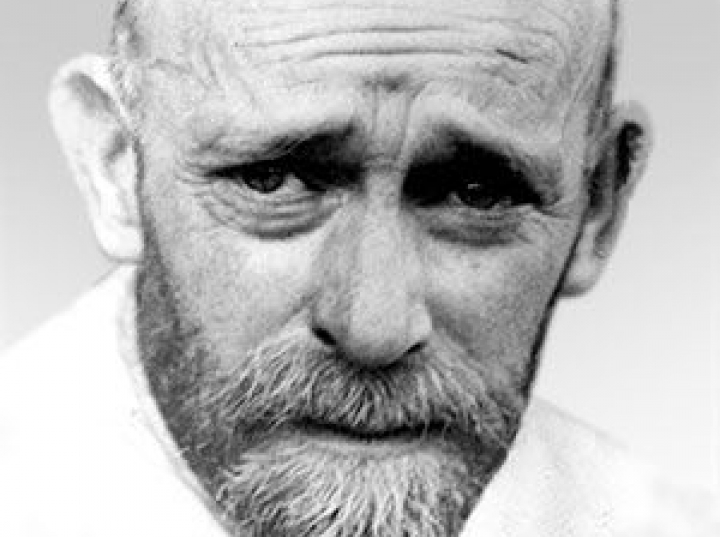
\includegraphics[width=10cm]{korczak}
		\caption{Janusz Korczak}
		Źródło: https://dzieje.pl/postacie/janusz-korczak (dostęp z dn. 13.01.2021)
	\end{figure}
	"Nauczycielu, bądź sobą,
	szukaj własnej drogi.
	Poznaj siebie, zanim zechcesz
	poznać dzieci"
	\par
	To słowa\cite{ref2} Janusza Korczaka, uznanego pedagoga, nauczyciela i wychowawcy. Spod jego pióra wyklarowało się kilka rodzajów wychowawcy. Wśród nich znajdziemy wychowawcę-apostoła, który intensyfikuje swoje wychowawcze działania zbyt szybko i bardzo emocjonalnie podchodzi do problemów swoich podopiecznych. Jest jeszcze wychowawca-dozorca, zdystansowany obserwator posiadający ścisły zbiór zasad w określonych sytuacjach, bacznie obserwujący poczynania uczniów. Wychowawca-tyran to bardziej despotyczna wersja jego poprzednika (dozorcy). Nie toleruje wszystkiego co wychodzi poza ramy jego surowych reguł. Z kolei wychowawca-liberał to przeciwieństwo piramidy autorytetu. Granica w relacji nauczyciel-uczeń jest sukcesywnie zamazywana przez wychowawcę liberalnego. Zachwiany zostaje autorytet nauczyciela, a postrzeganie go przez ucznia staje się upośledzone poprzez spoufalone zachowania wychowawcy. Wreszcie docieramy do dobrego wychowawcy, który rozumie problemy dzieci i jest w stanie je rozwiązać sposobami, które one same rozumieją i są chętne wprowadzić je w swoje życie. Dobrego nauczyciela cechuje pogodne nastawienie i charyzmatyczne zdolności do nawiązywania zdrowej relacji z uczniem.
	\par
	Wyzwaniem współczesnego nauczyciela jest według mojej połączenie cech wszystkich wymienionych typów nauczyciela i zachowanie balansu w zastosowaniu ich w kontaktach ze swoimi podopiecznymi. Dużo zależy od sytuacji i samego ucznia - każdy z nich wymaga indywidualnego podejścia do jego problemów. Idealny nauczyciel powinien potrafić szybko zidentyfikować jakim nauczycielem powinien się stać w tym konkretnym przypadku, aby w stu procentach zrozumieć i być w stanie pomóc dziecku.
	
	\subsection{Edukacja dzieci w wieku przedszkolnym}
	
	\par
	W tym podrozdziale skupię się na dzieciach w wieku przedszkolnym, ponieważ od najmłodszych lat można dostrzec schematy i utrwalanie pewnych zachowań w nauce podstawowych czynności takich jaki mówienie, pisanie czy postrzeganie świata. Józef Bednarek w swojej książce pod tytułem ‘Multimedia w kształceniu’\cite{ref3}, iż każdy uczeń chce się uczyć, ale to podejście pedagoga jest niezbędnym elementem, aby ta nauka ‘nie poszła w las’. Porównanie ww. autora, tablicy i kredy do telewizji i gier komputerowych wydaje się trafnym porównaniem podkreślającym rolę jaką odgrywa współczesny nauczyciel. Z pomocą przychodzi już wspomniana technologia. 
	\par
	Dzieci w wieku przedszkolnym tj. 3-6 lat są niezwykle wrażliwe na bodźce ze świata zewnętrznego. Przy oglądaniu zdjęć, obrazów, malunków ich mózg skupia się na rozpoznawaniu kształtów, kolorów, osób, a z wiekiem potrafi zauważyć analogię pewnych zestawień liter, kolorów, a nierzadko jest w stanie je nazywać. W swojej pracy wykorzystuje autorskie rozwiązanie interaktywnej kolorowanki w czasie rzeczywistym. Ów narzędzie opiera się na rozpoznawaniu kolorów, rysowaniu kształtów oraz stymuluje prawidłowy rozwój dziecka w myśl zasady - nauka poprzez zabawę. Zakresem badań będą przeprowadzenie serii eksperymentów i zapis obserwacji oraz wnioski z zachowań dzieci bawiących się wyżej opisanym narzędziem.
	\par
	Wracając do rozwoju dziecka w wieku przedszkolnym nie sposób zauważyć, że ten trzyletni okres jest na tyle ważny dla poprawnego zrozumienia świata, które dopiero co to dziecko poznało, że należy go podzielić na pewne etapy. Spotkałem się z podziałem na cztery etapy, ale skupię się na pierwszych trzech, gdyż uważam je za fundamentalne i kluczowe we właściwym procesie odbioru bodźców wysyłanych przez ten świat.
	\par
	Pierwsza faza jest typowo wrażliwa i cechuje się brakiem dostosowania się dziecka do otoczenia. Ma ono problemy ze zmianami zachodzącymi w jego życiu. Naturalnie w tej fazie dziecko jest najmniej samodzielne i wymaga ciągłej pomocy w podstawowych czynnościach.
	Faza druga to tak zwana. “faza pytań”. Dziecko nieustannie zadaje odpowiedzi czym zaznacza rozwój świadomości istnienia i coraz częściej potrafi samodzielnie wykonać rzeczy, których nie potrafiło w fazie pierwszej. W tej fazie najbardziej zauważalny jest postęp w mowie i rozwoju myślenia dziecka. Dodatkowym atutem dla rodziców (choć nie zawsze) jest wyraźne zaciekawienie dziecka elementami otoczenia czyli innymi słowy poszerzana jest przez dziecko wiedza o swoich zmysłach takich jak dotyk czy węch.
	\par
	Trzecia faza rozwoju dziecka w wieku przedszkolnym naznaczona jest drobnymi poleceniami do wykonania przez dziecko. Coraz śmielej podejmuje ono inicjatywę w niesieniu pomocy dorosłym, jest na tyle samodzielne, że nie wymaga ciągłego nadzoru dorosłego. Chętnie bierze udział w grach i zabawach, nie ma problemu z nawiązywaniem kontaktu z rówieśnikami. W tej fazie dziecko jest w stanie skoncentrować swoją uwagę na dłużej i nie stanowi to dla niego dużego problemu.
	\par
	Ostatnia faza to okres dziecka od około 5 do 7 lat, dlatego przyjęło się, że wówczas jest ono gotowe na podjęcie edukacji w szkole podstawowej. Dziecko jest na tyle samodzielne i potrafi rozwiązywać proste problemy, że jest w stanie słuchać poleceń nauczyciela i wspólnie pracować w grupie innym dzieci. Niewątpliwie bardzo dużo zależy od tego jak przebiegały wszystkie trzy fazy rozwoju dziecka. Czy miało ono wystarczająco dużo czasu na poprawne zinterpretowanie bodźców, czy jego rozwój stymulowany był w odpowiedni sposób przez rodziców. Zdarza się, że dziecko nie nadąża nad zmianami i potrafi “utknąć”, w którejś z trzech faz dlatego tak ważna jest obserwacja i pomaganie dzieciom w uczeniu się pewnych zachowań. Z pomocą przychodzą gry dydaktyczne, kolorowanki, a we wcześniejszych fazach zabawki sensoryczne pozwalające dziecku poznać siebie i swoje zmysły.
	
	
	
	\section{Multimedia w szkolnictwie}
	\subsection{Technologiczne BOOM}
	\par
	Przenieśmy się do roku 1945, właśnie dokonuje się przełom w dziedzinie cyfryzacji i komputeryzacji - pierwszy komputer ujrzał światło dzienne. Enigmatyczna nazwa ENIAC skłania nas do myślenia nad genezą tego słowa. W swojej istocie, nazwa ta, jest tak naprawdę banalna i pochodzi z języka angielskiego od ‘electronic numerical integrator and computer’\cite{ref4} czyli ‘elektroniczny integrator numeryczny i komputer’. Robi się ciekawiej. Warto w tym miejscu nakreślić ogólne pojęcie o  zautomatyzowanych procesach w 1945 roku. Mam na myśli to, jak ludzie postrzegali wówczas maszyny wykonujące skomplikowane obliczenia matematyczne w znacznie krótszym czasie niż oni sami. Ludzkość w późniejszych latach ‘40 ubiegłego wieku była sceptycznie nastawiona do robotów i maszyn. Głównie dlatego, że ich nie rozumieli - taka natura ludzka, że boimy się tego czego nie jesteśmy wyjaśnić w logiczny sposób.
	\par
	Dzisiaj tj. 80 lat później nie wyobrażamy sobie życia bez współczesnych rozwiązań techniki. Cóż, przynajmniej uważamy to za coś nierealnego, nieosiągalnego. Jak zauważa Monika Frania 'Człowiek żyjący na przełomie XX i XXI w. to świadek eksplozji przemian instrumentarium medialnego'\cite{ref5}. Ciężko się nie zgodzić. Nasi dziadkowie pamiętają czasy, w których technologia była im zupełnie obca. Ba, sami doświadczyliśmy okresu, w którym ‘Internet’ było słowem obcym, niezrozumiałym. Czym jest tak naprawdę ta cała ‘technologia’, o którą się tu rozchodzi? Według Polskiego Słownika PWN\cite{ref6} słowo ‘technologia’ opiera się na metodach powiązanych z procesem przetwórczym lub produkcji. Technologie informacyjne jako termin są z nami stosunkowo od niedawna. Wraz ze wzrostem znaczeń maszyn i komputerów, przez gromadzenie i agregację danych, aż do ‘targetowania’ użytkowników wspomnianego już Internetu, na znaczeniu zyskały również inne dziedziny nauki, ale i nie tylko.
	\par
	Z biegiem lat zauważamy coraz to nowsze rozwiązania technologiczne wprowadzane począ- wszy od szkół podstawowych, a skończywszy do szkolnictwie wyższym. Kiedyś hitem były tablice multimedialne, które stawały się niemalże wizytówką placówki oświatowej. Tak było kilka lat temu. Rok 2020 okazał się jeszcze bardziej wymagający i zmusił szkoły, organy oświatowe a także samorządy i placówki administracyjne do zakupu wszelkiego rodzaju tabletów, laptopów, notebooków, smartfonów etc. Nagle okazało się, że podstawowy ekwipunek ucznia o wadze 11 kilogramów został zastąpiony jednym 800g tabletem, w którym znajdują się elektroniczne wersje niezbędnych do nauki podręczników i ćwiczeń. W przedszkolach również zauważa się wzrost technologii wykorzystywanej do nauki dzieci. Co prawda komputery już wcześniej były obecne w salach zabaw, a dzieci potrafiły w mniej lub bardziej logiczny sposób wyjaśnić obecność elektroniki, ale elektroniczna kolorowana to coś całkiem nowego dla całego półświatka przedszkolnego. Cofnijmy się jednak o kilkanaście lat wstecz do momentu, w którym kształtował się termin ‘mediów’ w kontekście elementów niezbędnych do prowadzenia dydaktyki szkolnej. Bywało, że oba terminy były używane zamiennie, lecz nie każdy potrafił, z całkowitą pewnością, wyjaśnić dlaczego tak się dzieje i jakie są różnice, o których mało kto wiedział. Eugeniusz Kameduła\cite{ref7}, mając na myśli tamte czas pisał: “[...] używa się często terminu media zamiast polskiego słowa środki. W dydaktyce termin ten odnosi się do różnorodnych przedmiotów oryginalnych lub ich desygnatów obrazowych, dźwiękowych, obrazowo- dźwiękowych lub manipulacyjnych, które umiejętnie zastosowane w procesie kształcenia mogą ułatwić poznawanie nowych wiadomości, przyczyniać się do kształtowania umiejętności i nawyków. Dlatego też jest stosowana nazwa dwuczłonowa - środki dydaktyczne, którymi mogą być materiały dydaktyczne jako nośniki treści, a czasami także pewne urządzenia techniczne będące źródłem informacji. Niektórzy dydaktycy środkami nazywają urządzenia techniczne, umożliwiające projekcję lub transmisję materiałów dydaktycznych (na przykład radio, telewizor, aparat fotograficzny i tym podobne), co wprowadza pewien chaos w klasyfikacji środków dydaktycznych”
	\begin{figure}
		\centering
		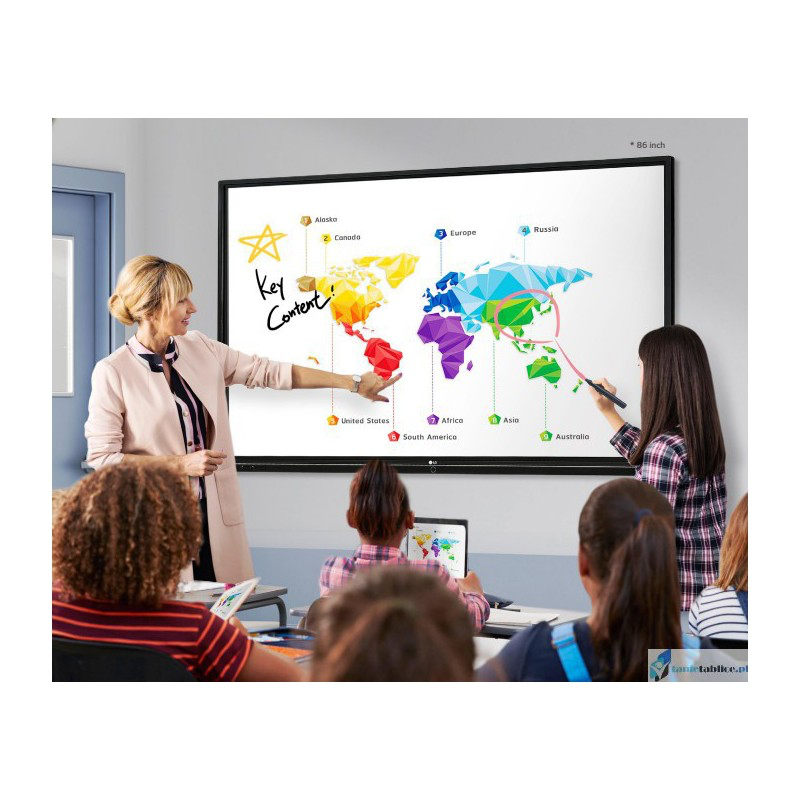
\includegraphics[width=10cm]{modern_school}
		\caption{Interaktywna szkoła}
		Źródło: https://www.digitalavmagazine.com/2019/12/16/lg-presenta-sector-educativo-y-corporativo-nueva-pantalla-interactiva-tactil/ (dostęp z dn. 29.01.2021)
	\end{figure}
	\par
	Żyjemy w czasach, w których korzystanie z takich narzędzi jest na tyle powszechne, że jesteśmy w stanie podzielić je na kategorie\cite{ref8}:
	\newline
	\begin{itemize}
		\item Gry komputerowe, dzięki którym dziecko poszerza swoje umiejętności i wiedzę
		\item Zabawy komputerowe mające na celu oswojenie dziecka z obsługą maszyny
		\item Zadania komputerowe jako nowoczesna forma tradycyjnych ćwiczeń edukacyjnych
		\item Programy informacyjne czyli elektroniczne wersje słowników, encyklopedii czy narzędzia do tworzenia prezentacji
		\item Programy użytkowe takie jak edytory grafiki, tekstu, dźwięku i tak dalej
	\end{itemize}
	\par
	Nauka nowych rzeczy przez dzieci w wieku przedszkolnym może odbywać się na różne sposoby - poprzez przeżywanie, aktywne działanie i sprostanie napotkanym problemom. Nowoczesne metody nauki z wykorzystaniem technologii muszą odbywać się zgodnie z podstawą programową, według której stymulowany jest rozwój dziecka. Mówi o tym podstawa programowa, której fragment odnośnie opisu dziecka, które pokonało kolejne szczeble edukacji brzmi: “dziecko kończące wychowanie przedszkolne interesuje się urządzeniami technicznymi (na przykład używanymi w gospodarstwie domowym), próbuje rozumieć ich działanie i zachowuje ostrożności przy korzystaniu z nich”\cite{ref9}. Do jednym z najważniejszych celów nauczania przedszkolnego jest “umiejętność posługiwania się nowoczesnymi technologiami informacyjno-komunikacyjnymi w tym także dla wyszukiwania i korzystania z informacji”. Nie ucieknie się od rzeczywistości, która kreuje u dzisiejszych dzieci poczucie wyalienowania. Często bywa, że świat realny z wyimaginowanym przez szeroko pojęte multimedia przenika się i zakłóca prawidłowy rozwój dziecka. Bardzo ważnym jest, aby nauczyciel odpowiednio dobierał dostępne narzędzia i urozmaicał naukę poprzez mieszanie rodzajów nauki, o których pisałem wyżej.
	
	\section{Technologie wykorzystywane w analizie obrazów}
	\subsection{C/C++}
	Zapewne każdy aspirujący programista musiał miał styczność z tym językiem. Prosty, niewy- magający, wybaczający błędy - idealny do rozpoczęcia przygody z programowaniem. Język C++ to nie jest “związek” tylko na chwile. Jego zastosowanie można zaobserwować w takich produktach jak Windows, Mac OS, pakiet Adobe czy Office. Dlaczego? Odpowiedź jest prosta - język C++ jest bardzo wydajny i zużywa o wiele mniej zasobów przy kompilacji. Jak słusznie zauważa Karol Kuczmarski w swojej książce “Kurs C++. Od zera do gier kodera” \cite{ref10} mocnym atutem języka C++ jest jego popularność i dostępność rozwiązań. Cytując jego słowa można stwierdzić, że “[...] C++ zdaje się być bardziej uniwersalny (od języka Delphi, przyp. tłum.). Dobrze rozumie się z ważnymi dla nas bibliotekami graficznymi, jest także bardzo szybki i posiada duże możliwości” Jak to się stało, że język C++ osiągnął taką przewagę nad innymi językami? Żeby odpowiedzieć na to pytanie należy cofnąć się do początków lat siedemdziesiątych kiedy to niejaki Dennis Ritchie finalnie zaimplementował z pomocą języka C jądro systemu operacyjnego Unix. Uznaje się to wydarzenie za początek dominacji języka C (i jego późniejszych ewolucji, o których 
	wspomnę w dalszej części). Po roku 1980 język C (a także jego późniejsza wersja z dwoma plusami) wiódł prym w programowaniu systemów i aplikacji czego dowodem był produkt Microsoftu pod nazwą Windows, przy którego budowanie w znacznej mierze opierano się na wyżej wymienionym języku programowania. Warto zaznaczyć, że język C/C++ posiadał bardzo ważną cechę jaką niewątpliwie jest możliwość przenoszenia go na inne urządzenia. Dodatkowym atutem, o którym trzeba powiedzieć jest to, że większość dzisiejszych sterowników do kart graficznych, dźwiękowych i tak dalej są pisanie niskopoziomowo z wykorzystaniem właśnie języka C/C++.
	\subsection{Python}
	Drugim językiem, który jest w pewnym sensie zamiennikiem w kontekście nauki programowania jest język Python. Powiedzieć, że Python i C/C++ to dwa różne języki to powiedzieć o wiele za mało. Na wstępie dodam, że pierwszy z nich jest językiem interpretowanym, natomiast drugi kompilowanym. Co to oznacza dla programisty? Niewiele. Jakby spytać maszyny, na którym “odpalane” są fragmenty kodu? Bardzo dużo. Języki interpretowane muszą być “przetłumaczone” na język zrozumiały dla maszyny. Oczywiście zajmuje to dodatkowy czas, a w programowaniu głównie chodzi o to, żeby zrobić dużo w jak najkrótszym odstępie czasowym. Język C/C++ ma od razu strukturę języka kompilowanego czyli takiego, który nie wymaga dodatkowego czasu na przekładanie na język “maszynowy”. Python jest prostym językiem, ale z ogromnymi możliwościami. Główną zaletą jest szybkość pisania kodu i prostota w wytwarzaniu oprogramowania. Czytelność składni również jest mocną stroną tego języka. Początkujący programista, który zna podstawy Python’a jest w stanie wytworzyć program gotowy do uruchomienia w konsoli, programie graficznym, stronę internetową czy po prostu niewielki skrypt z niezbyt skomplikowanym zadaniem do wykonania (choć oczywiście zdarzają się, i to nie rzadko, skrypty z setkami linijkami kodu).
	\par
	Python posiada niezliczoną ilość bibliotek do rozwiązywania bardzo różnych problemów. Tensorflow do sztucznej inteligencji, Keras do sieci neuronowych, Matplotlib do wykresów i diagramów i w końcu OpenCV, na którym opiera się część praktyczna niniejszej pracy (choć zaimplementowana w języku C++). Skupmy się na tej ostatniej, a więc bardzo popularnej bibliotece do przetwarzania i analizy cyfrowej obrazów przechwyconych \linebreak na przykład z kamery komputera. Pomysłodawcami biblioteki byli programiści Intel’a, a sama biblioteka jest wieloplatformowa czyli dostępna na trzy najbardziej powszechne systemy operacyjne - Windows, Linux i MacOS. Technologie lub języki programowania, przy użyciu których można wykorzystać bibliotekę OpenCV, są ogólno dostępne i są nimi:
	\newpage
	\begin{itemize}
		\item C/C++, C Sharp
		\item Python
		\item Java
		\item NodeJS
	\end{itemize}
	O możliwościach i procesie przetwarzania kodu przez wyżej wymienioną bibliotekę wspomnę w dalszej części pracy przy okazji wyjaśniania dokładniej zagadnienia przetwarzania \linebreak cyfrowego obrazów w czasie rzeczywistym.
	
	\subsection{Ewolucji ciąg dalszy czyli język C Sharp (C#)}
	W końcówce lat dziewięćdziesiątych zaczęto zastanawiać się na stworzeniem od podstaw języka programowania opartego na obiektowości, który mógłby rywalizować z zyskującą popularność Javą. Narodził się pomysł utworzenia zespołu projektowego, którego zadaniem byłoby stworzenie mocnego konkurenta na “rynku obiektowości” w myśl zasady głoszonej przez model PME (Properties - Methods - Events). Na czele projektu stanął charyzmatyczny Duńczyk Anders Hejlsberg - znany i ceniony programista w środowisku informatycznym. W swoim dorobku miał doświadczenie w pracy nad takimi językami jak wspomniany już wcześniej Delphi, Pascal, a później również TypeScript. W swojej książce pod tytułem “The C\# Programming Language” \cite{ref11} wspominał, że praca przy nowym języku była dla niego nie lada wyzwaniem, ale zaznaczył, że traktował to jako ciekawą rozrywkę, żeby nie powiedzieć zabawę. Dodał, że miarą rozwiązywania problemów jest dodanie wartości tworzonemu produktowi przy poszukiwaniu solucji.
	\subsection{C/C++ versus C Sharp}
	\begin{figure}
		\centering
		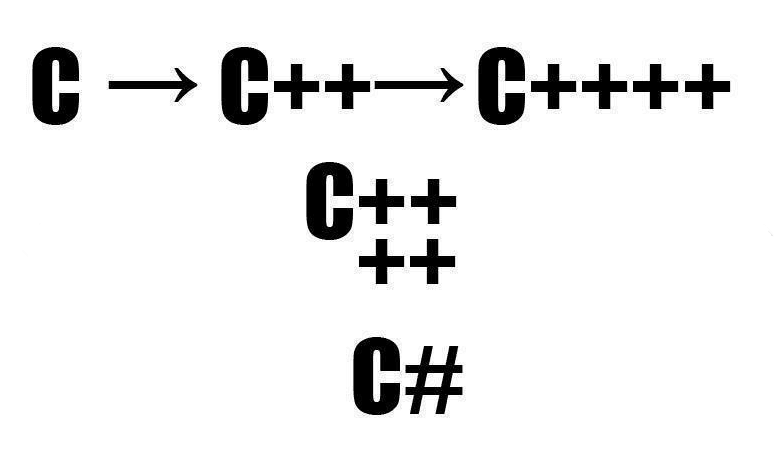
\includegraphics[width=10cm]{cvscsharp}
		\caption{Geneza identyfikacji wizualnej języka C}
		Źródło: https://i.imgur.com/jSVx4kF.png (dostęp z dn. 03.03.2021)
	\end{figure}
	\par
	Mając na uwadze projekt wykorzystany w badaniach nad niniejszą pracą postaram się skonfrontować starszą wersję języka C/C++ oraz jego “ulepszoną” wersję “z krzyżykiem”. Na początku garść historii. Język C Sharp jest dosłownie rozwinięciem jego poprzednika. Jak się dobrze przyjrzeć, na symbol hashtagu w nazwie składają się cztery plusy co ma być sygnałem dla programistów w C++, że C Sharp jest bogatszą i lepszą wersją tego co już znają. Czym tak naprawdę się różnią? Jest wiele składowych, ale zacznijmy od początku.
	\par
	Po pierwsze, jak już wcześniej wspomniałem, język C/C++ jest językiem kompilowanym, który przetworzy go nam na język binarny czyli zrozumiały dla maszyny. Pliki ze skompilowanym językiem C/C++ mają rozszerzenie *.exe. Podobnie jest w przypadku C#, jednak z tą różnicą, że nim język zacznie być kompilowany na “binarkę” maszyna musi “zaciągnąć” i skompilować wszystkie załączone biblioteki i wtyczki, które są niezbędne przy uruchamianiu kodu napisanego w C Sharpie. Pliki wykonawcze kodu C# są cięższe niż te napisane w C/C++.
	\par
	Po drugie, programy wykorzystujące kod napisany w C/C++ są zwykle szybsze. Wykorzystuje je się w momencie, w którym zależy nam na jak największej optymalizacji kodu z równoczesną wysoką wydajnością bez spadków wartości wykorzystania CPU. Przykład? Aplikacje, których zadaniem jest analiza łączy internetowych w ogólnym pojęciu wykorzystuje właśnie aplikacje napisane w języku C/C++.
	\par
	Po trzecie, programista C# nie musi martwić się o zwalnianie alokowanej pamięci, ponieważ wbudowane narzędzie o nazwie “garbage collector” zwalnia twórcę z obowiązku monitorowania wykorzystanej pamięci i w razie potrzeby zwalniania tej niepotrzebnej lub wykorzystanej. C/C++ niestety takiego narzędzia nie posiada i wymaga się od programisty ciągłego zwalniania zbędnej pamięci.
	\par
	Czwartym elementem jest wieloplatformowość lub jej brak. W przypadku programów napisanych w C/C++ jesteśmy w stanie skompilować i uruchomić je w środowisku Windows, Linux lub MacOS. Choć obecnie coraz głośniej mówi się o wieloplatformowości w kontekście C Sharp’a to wciąż jest on zarezerwowany tylko dla środowiska autorstwa jego twórcy - Microsoftu i jego sztandarowemu produktowi, systemowi operacyjnemu Windows.
	\section{Programowanie GPU}
	\subsection{Procesory graficzne}
	Jak wspomniałem jedną z zalet języka C/C++ jest szeroki zasób i dostępność do bibliotek o bardzo różnym charakterze. Od napisania mikrokontrolera przez fotokomórkę aż po grę komputerową. W dzisiejszym świecie coraz więcej elementów otaczającego nas świata zależy właśnie od technologii. Częściej musimy zasięgnąć opinii przysłowiowych “informatyków”, aby Ci wytłumaczyli nam chociażby jak kupić bilet na autobus z poziomu telefonu komórko- \ wego. Wraz z rozwojem sektora oprogramowania graficznego na znaczeniu, w kwestii mocy obliczenio- \ wej, zyskały układy graficzne oparte głównie na dwóch architekturach - NVIDIA CUDA oraz OpenCL. Zauważono, że obecnie układy te pozwalają na wykonanie serii bardziej skomplikowanych operacji niż dotychczas sądzono. Nowoczesne procesory graficzne są w stanie generować żądany obraz w czasie rzeczywistym i co więcej są w stanie zmodyfikować go według określonych zasad ustanowionych przez programistę. Dzieje się tak, gdyż układ CPU komunikuje się z układem GPU z pomocą specjalnego API (Application Programming Interface) w charakterze komunikatora pomiędzy dwoma układami. Poniższy schemat powinien nieco rozjaśnić powyższe rozważania.
	\begin{figure}
		\centering
		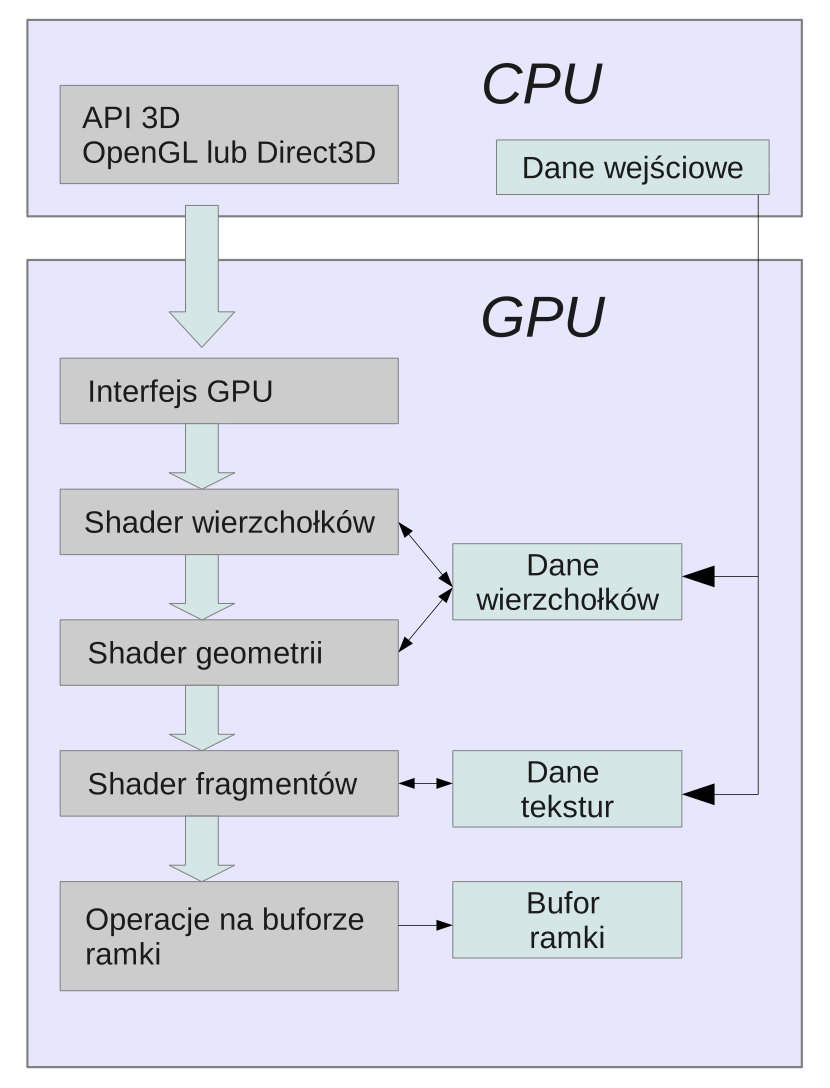
\includegraphics[width=10cm]{gpu}
		\caption{Schemat komunikacji CPU z GPU za pomocą API}
		Źródło: https://i.ibb.co/dfVbgJW/gpu.png (dostęp z dn. 22.02.2021)
	\end{figure}
	\par
	Dzięki takiemu rozwiązaniu powszechne stało się wykorzystanie mocy obliczeniowej procesorów graficznych w tworzeniu oprogramowania wykorzystującego funkcje przetwarzania obrazu przechwyconego z kamery. Przykładem takiego rozwiązania jest na przykład rozpoznawanie twarzy w nowoczesnych telefonach, skanowanie numerów rejestracyjnych \linebreak samochodów wyjeżdżających z parkingów, algorytmy rozpoznawania elementów na obrazie w celu identyfikacji i opisania rzeczy znajdujących się przed obiektywem kamery. W nowych samochodach można znaleźć system odpowiadające za śledzenie toru, po którym porusza się pojazd, albo oprogramowanie odpowiadające za detekcję znaków drogowych i stosowanie odpowiednich ograniczeń wbudowanych w oprogramowanie komputera pokładowego. Można by wymieniać i wymieniać, ale żeby “namacalnie” (a przynajmniej w teorii) móc poczuć wcześniej wspomniany skok technologiczny warto chociażby zdobyć i porównać zdjęcia dwóch gier wideo, których daty premier oddalone są na osi czasu o raptem 20 lat. W ciągu tak krótkiego czasu zrobiono więcej niż przez ostatnie 50 lat w kwestii motoryzacji (chociaż Elon Musk każe sądzić inaczej). Jestem bardzo ciekaw jak będzie wyglądać rozgrywka za drugie tyle lat. Prawdopodobnie niemożliwym zadaniem będzie odróżnienie gry od rzeczywistości.
	Sekretem realistycznej grafiki w grach komputerowych jest skomplikowanie algorytmów odpowiedzialnych za renderowanie w czasie rzeczywistym tekstur w bardzo wysokiej rozdzielczości. Swoim artykule Christoph Liedtke z redakcji GameStar (gamestar.de) \cite{ref12} zwraca szczególną uwagę na nowe efekty graficzne, które pojawiły się wraz z rozwojem mocy obliczeniowej kart graficznych “Również efekty graficzne takie jak np. mapowanie wypukłości (bump mapping), multiteksturowanie czy też oparta na rzeczywistych obrazach technika fotogrametrii, a także pakiety tekstur o wysokiej jakości tworzone przez fanów, sprawiają że pod względem graficznym gry stają się coraz bardziej imponujące.”\\
	\begin{figure}
		\centering
		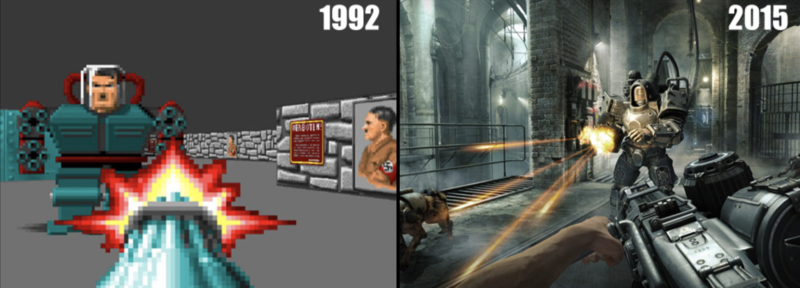
\includegraphics{grafika}
		\caption{Porównanie gier wideo kiedyś a dziś}
		Źródło: https://www.gry-online.pl/S018.asp?ID=1721 (dostęp z dn. 09.03.2021)
	\end{figure}
	\par
	Początkowo jednostki GPU były tworzone z myślą o statycznym przetwarzaniu jedynie danych przychodzących. W ten sposób programiści nie mieli realnej możliwości na większą ingerencję w działanie tych układów. Dużo zmieniło się pod koniec roku 1999, kiedy na rynek weszły pierwsze układy o nazwie T&L (transform and lighting)\cite{ref13}. Były one odpowiedzialne za renderowanie obrazów trójwymiarowych przedstawionych na siatce dwuwymiarowej Poniższy obraz powinien wyjaśnić pojęcie Transform & Lighting i zasady jego działania:
	\begin{figure}
		\centering
		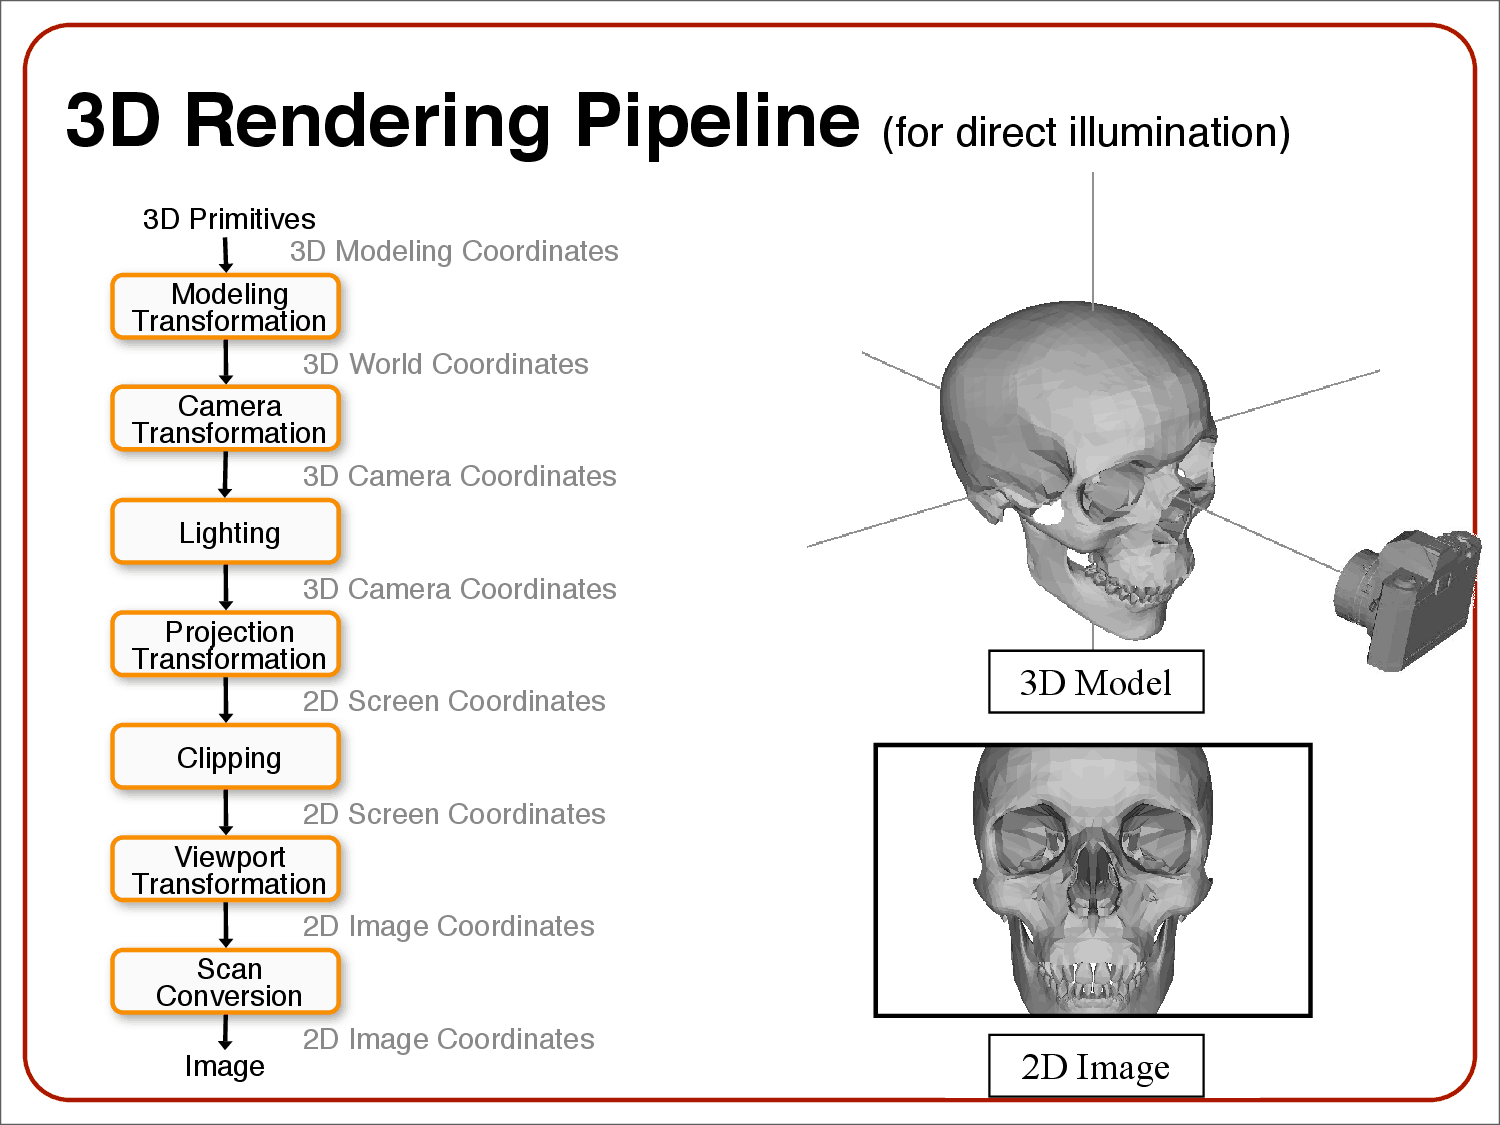
\includegraphics[width=15cm]{tandl}
		\caption{Transform Lightning}
		Źródło: https://www.youtube.com/watch?v=BUcch9b6cFg (dostęp z dn. 16.04.2021)
	\end{figure}
	\par
	Na początku, na podstawie współrzędnych x, y, z (przyjąłem standardowe przedstawienie osi współrzędnych w trójwymiarowej przestrzeni - równie dobrze mogłyby być to inne oznaczenia, ale przyjęło się używanie trzech powyższych) określa się ich położenie względem współrzędnych “świata”, w którym mogą istnieć inne obiekty posiadające swoje współrzędne w przestrzeni lokalnej. Proces ten jest nazywany rzutowaniem obiektów na scenę i nosi nazwę z języka angielskiego modeling/geometric transformations.
	\par
	Następnym ważnym krokiem jest nadaniem obiektom kolorów. Postrzeganie kolorów jest uwarunkowane przez odbiór sygnałów przez nasz zmysł wzroku. Jest to pewnego rodzaju gra i zabawa, która czasami przyprawia o ból głowy spowodowany zbyt dużą ilością \linebreak wysyłanych sygnałów przez obiekt, na który patrzymy (na przykład iluzja optyczna). W zależności od częstotliwości wysyłanego sygnału jesteśmy w stanie ocenić czy obiekt na który patrzymy znajduje się blisko, daleko lub w jakiej pozycji jest do nas zwrócony. O postrzeganiu barw mówi prawo fizyki, a dokładniej jej część zwana prawem optyki. W celu uzyskania więcej informacji na ten temat zachęcam do obejrzenia programu pod nazwą “Pułapki umysłu” emitowany przez stację telewizyjną National Geographic.
	\par
	W dalszej części renderowania ustala się projekcję obrazu, na przykład ustawiając kadr, który będzie rejestrować kamera. Elementy, które nie znajdą się w granicach wyznaczonego przez ten kadr są usuwane, a proces ten nazywa się clippingiem (z języka angielskiego “wycinanie”).
	\par
	Jednym z ostatnich etapów jest tak zwany scan conversion lub bardziej “polska” nazwa rasteryzacja obrazu. Mając współrzędne obiektu jesteśmy w stanie wyznaczyć proste, które przechodzą częściowo przez te punkty, co pozwala na zaznaczenie danego obszaru czyniąc częścią efektu końcowego.
	\begin{figure}
		\centering
		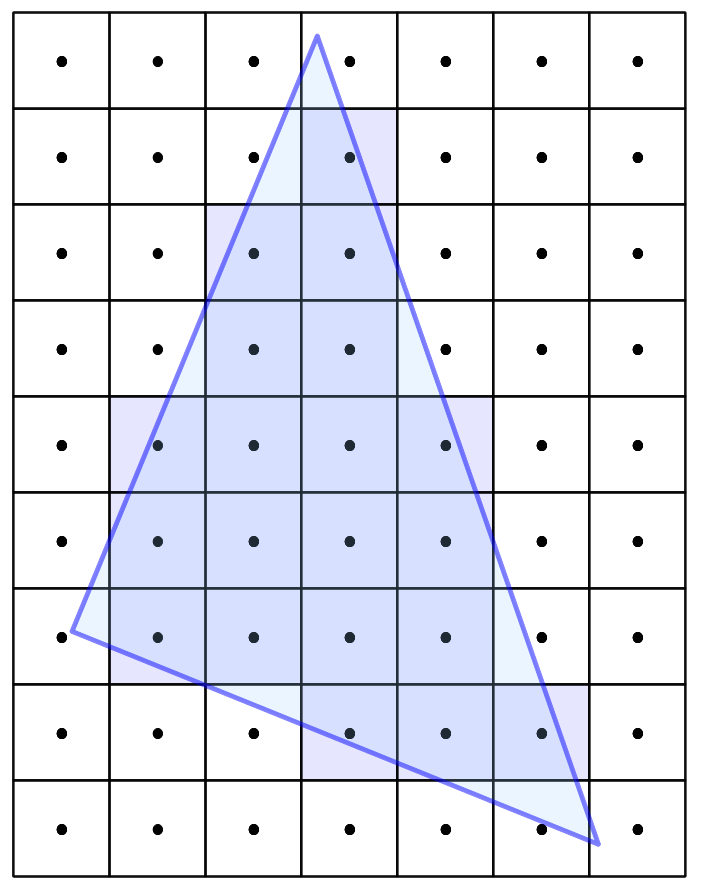
\includegraphics[width=15cm]{polygon}
		\caption{Schemat rasteryzacji obrazu}
		Źródło: https://i.ibb.co/dfVbgJW/gpu.png (dostęp z dn. 22.02.2021)
	\end{figure}
	\par
	Wracając do układów opartych na powyższym procesie ich znaczenie na rynku \linebreak zostało zachwiane rok później w momencie wprowadzenia API DirectX w wersji 8.0 tak zwanych shaderów. Dało to ogromne możliwości programistom chcących wprowadzać własne zmiany w konfigurację układów GPU, które od teraz stały się bardziej programowalne niż kiedykolwiek. Deweloperzy mogli tworzyć skomplikowane obliczenia matematyczne na wierzchołkach wyżej wymienionej sceny, a także na finalnym wyniku procesu T\&L. Fragmenty kodu odpowiedzialne za powyższe zadania były wykonywane przez specjalnie do tego stworzone jednostki strumieniowe wbudowane w układ graficzny o architekturze SIMD.
	\par
	Tutaj dochodzimy do sedna tego podrozdziału bo od tego momentu programiści zaczęli rzutować problemy naukowe na algorytmy liczone przez układy GPU, które od tej pory nazywały się General-Purpose Computing on Graphics Processing Units, czyli w skrócie GPGPU. Oczywiście GPU to nie to samo co GPGPU, różnicą jest cel do jakich stosuje się wyżej wymienione układy. Te pierwsze wciąż były odpowiedzialne za rendering obiektów i wyświetlanie wizualnej części programów na monitorach komputerowych (w bardzo dużym skrócie). General-Purpose Computing on Graphics Processing Units stosowano stricte do skomplikowanych algorytmów, które w oparciu o potężną moc obliczeniową swoich podzespołów potrafiły wyliczać wynik szybciej niż dotychczasowe jednostki CPU, na których ciążyła odpowiedzialność za cały system operacyjny. Może ktoś zapyta, ale zaraz, jak układ graficzny, który do niedawna wyświetlał i kolorował figury w trójwymiarze jest w stanie rozwiązywać naukowe problemy? Na początku API OpenGL pozwalało na rysowanie \linebreak trójkątów i wielokątów w trójwymiarze, ale też w dwuwymiarowym świecie. Nijak ma się to do prawdziwych barier na jakie często trafiały osoby na co dzień zajmujące się nauką o świecie. Dlatego w dwa tysiące trzecim roku, pewna grupa naukowców z Uniwersytetu Stanforda mieszczącego się w Dolinie Krzemowej skonstruowała całkiem nowy model wykorzystujący GPGPU do zarządzania zasobami obliczeniowymi układu graficznego. Wspominany już w tej pracy język C przyczynił się niejako do powstania tego modelu, bowiem idealnie nadawał się do zaprogramowania kontrolerów i zainicjowania całkiem nowych sterowników w układach GPGPU. Paweł Pięta w swojej pracy pod tytułem “Współczesne architektury procesorów graficznych” tak podsumował zdolności układów graficznych na początku dwudziestego pierwszego wieku: “Napędzane nienasyconym zapotrzebowaniem rynku na wysokiej jakości grafikę 3D, programowalne procesory graficzne ewoluowały w wysoce równoległe, wielowątkowe, wie- lordzeniowe procesory z ogromną mocą obliczeniową i bardzo dużą przepustowością pa- mięci. Są projektowane w taki sposób, aby więcej tranzystorów było w nich poświęconych przetwarzaniu danych, aniżeli ich buforowaniu, czy kontroli sterowania, co schematycznie pokazuje rysunek”
	\begin{figure}
		\centering
		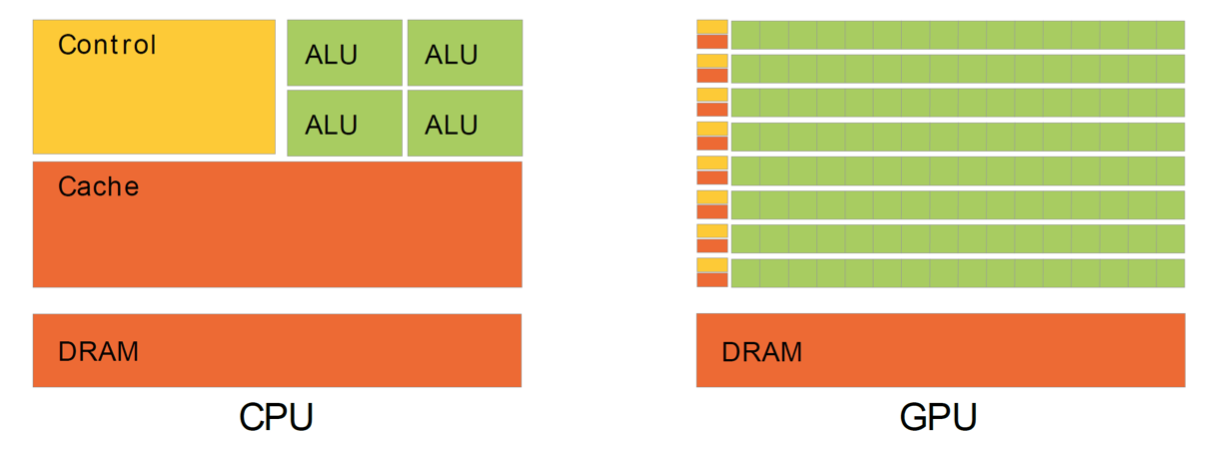
\includegraphics[width=15cm]{simd}
		\caption{Porównanie schematów CPU a GPU}
		Źródło: [13]
	\end{figure}
	\subsection{Cyfrowa przedstawienie fotografii}
	Aby wyjaśnić sposób działania algorytmów odpowiedzialnych za analizę fotografii czy obrazu z aparatu/kamery trzeba nieco cofnąć się w czasie do klasycznej fotografii.
	W czasach, gdy ludzie chcieli upamiętnić ważną chwilę trudno szukać jako takiej technologii znanej nam dzisiaj. Czy można powiedzieć, że wraz z rozwojem fotografii cyfrowej, wymyślono aparat na nowo?. O tym za chwilę. Na ten moment zostańmy jeszcze chwilę w tematach, jak to się dziś ładnie mówi - retro. Klasyczne, żeby nie powiedzieć stare, aparaty fotograficzne działają w oparciu o nośniki wykorzystujące materiały światłoczułe (np. klisze). Trzeba zaznaczyć, że klasyczny nie jest równy analogowy. W rozumieniu analogowy mamy na myśli te, które nie wykorzystują sygnału cyfrowego do zapisu obrazu na materiale światłoczułym. Błędne określenie aparatów analogowych klasycznymi pojawiło się wraz z rozwojem fotografii cyfrowej. Trzeba z tego zapamiętać tyle, że w dawnych aparatach klasycznych nie stosowano zapisu obrazu za pomocą sygnału analogowego. Tymczasem świat poszedł naprzód, a to co najważniejsze, ludzie zaczęli “zapamiętywać” swoje życie na cyfrowych matrycach nowoczesnych aparatów. Cyfrowy zapis od analogowego różni się tym, że w tym pierwszym fotografia utrwalana jest binarnie na matrycach cyfrowych, które po błyskawicznym “przetłumaczeniu” oddaje obraz w różnych barwach reprezentowanych przez ciąg zero-jedynkowy. Każdy taki obraz składa się z setek, tysięcy pikseli. Każdemu pikselowi odpowiada konkretny obszar i zapis na ww. cyfrowej matrycy. Innymi słowy, działanie aparatu takie same, ale zapis już niekoniecznie. Mając zapis binarny zdjęcia możemy dzięki algorytmom zastosować szereg operacji mających na celu np. rozpoznanie tekstu, detekcję ruchu, zliczanie elementów czy wspomnianą już wcześniej asystę dla kierowcy przy zjeździe z pasa na jezdni. Maszyna mając zero-jedynkowe przedstawienie fotografii widzi macierz liczb, która zawiera reprezentację barw.
	\begin{figure}
		\centering
		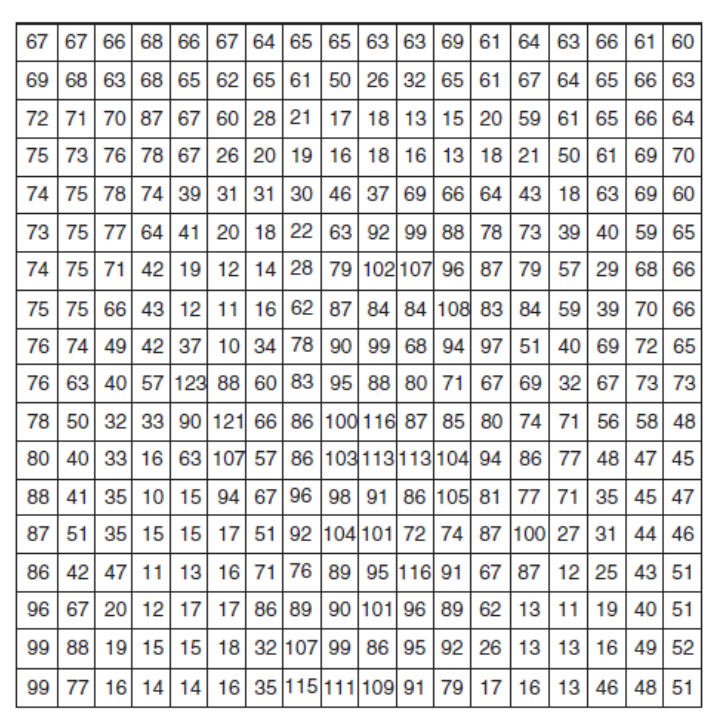
\includegraphics[width=10cm]{macierz}
		\caption{Macierz liczb reprezentująca barwy}
		Źródło: [14]
	\end{figure}
	Jest to jedna ze struktur obrazów cyfrowych, które “rozumie” maszyna. W głębszym rozumieniu, pozyskiwanie obrazów cyfrowych i translację ich na język komputerowy nazywamy dyskretyzacją obrazu. Ryszard Tadeusiewicz i Przemysław Korohoda w “Komputerowej analizie i przetwarzanie obrazów” \cite{ref14} zaznaczają, że ów sztuczna reprezentacja i sposób jej kreowania posiada swoje ograniczenia wynikające z wydajności dzisiejszych maszyn. Niestety (a może i stety) nie osiągnęliśmy jeszcze poziomu maszyn, które można byłoby określić szybszymi i mądrzejszymi niż zmysły ludzkie (w tym wypadku mam na myśli zmysł wzroku). Na ten moment uważa się, że przybliżone przetwarzanie danych w czasie rzeczywistym przez ludzkie oko plasuje się na poziomie około stu megabajtów na sekundę co przekracza możliwości komputerów w znanym nam świecie. Być może, a raczej wielce prawdopodobne, jest to, że maszyna oparta o technologię kwantową sprostałaby wyżej wymienionym wymaganiom, ale na tę chwilę musimy te rewelacje odsunąć na bok i skupić się nad dostępnością dzisiejszych rozwiązań. Co możemy zrobić, aby ograniczyć reprezentację obrazu? Ryszard Tadeusiewicz i Przemysław Korohoda wymieniają między innymi możliwość ograniczenia fotografii poprzez zmniejszenie ilości szczegółów, ale też uproszczenie i ujednolicenie stanów elementów (na przykład poprzez wykorzystanie czarno-białej palety barw). Autorzy sugerują również analizowanie obrazu płaskiego zamiast przestrzennego i statycznego zamiast dynamicznego. Ten ostatni przypadek odnosi się do ciągu klatek (obrazów) dlatego w dalszej części nie będę go brał pod uwagę. Warto mieć to jednak na uwadze. Dzisiejsze algorytmy przetwarzające fotografie wykorzystują jeden z dwóch sposobów umieszczenia cyfrowych odpowiedników elementów obrazu (pikseli). Są to: heksagonalne i kwadratowe.
	\begin{figure}
		\centering
		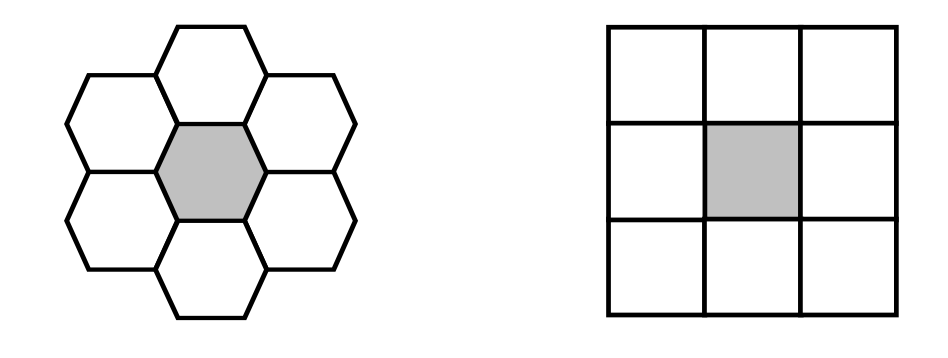
\includegraphics[width=15cm]{dyskretyzacja}
		\caption{Różne sposoby dyskretyzacji obrazu}
		Źródło: [14]
	\end{figure}
	Wspomniana macierz reprezentująca barwy, a dokładniej nasycenie jednej z trzech bar modelu RGB (Red - Green - Blue), służy komputerowi jako źródło kilku istotnych danych. Maszyna rozpoznaje nasycenie, barwę oraz potrafi rozpoznać co znajduje się na pierwszym, drugim planie i tak dalej. Niemniej jednak to wciąż za mało, aby być pewnym otrzymanych wyników. Na dane wejściowe nierzadko stosuje się szereg zabiegów mających na celu zniwelowanie niedoskonałości powstałych przy wykonywaniu fotografii.
	Zanim jednak zajmiemy się wyżej wymienionymi operacjami należy sobie wyjaśnić z czego biorą się błędny przy pracy ze źle przygotowanymi danymi wejściowymi. Niestety czynnik ludzki ma tutaj ogromne znaczenie dla wysokiej wartości tych danych. Często nie przywiązujemy należytej uwagi do jakości aparatów i ich podzespołów co prowadzi od początku do niewystarczającej ostrości, naświetlenia i tym podobne. Również pośpiech nie jest dobrym doradcą w tych sprawach. Ważną cechą dobrego zdjęcia jest odpowiednie światło i ostrość - co w przypadku obiektów poruszających się jest niezwykle utrudnione, żeby nie powiedzieć niemożliwe. 
	\subsection{Operacje na fotografiach}
	Usuwanie szumu z fotografii nie jest czymś nowym. Zasada działania algorytmów “odszumiających” jest całkiem prosta w wytłumaczeniu. Jak wcześniej wspomniałem, komputer widzi obraz jako macierz z setkami małych punktów (pikselami). Filtr odpowiedzialny za usuwanie szumu sprawdza każdy element fotografii i jej bliskie sąsiedztwo analizując wartości pikseli. Założeniem jest to, że każdy punkt o przybliżonej barwie, naświetleniu powinien mieć podobne wartości, a każde odchylenie od tej reguły traktowane jest jako niepożądane zachowanie i modyfikowane w zależności od parametrów “dobrych pikseli”. Metody usuwania szumu są dwie - poprzez średnią arytmetyczną i medianę. W przypadku pierwszej filtr nadpisuje analizowany obszar wartościami średnimi obliczonymi na podstawie barwy i ostrości. W drugiej metodzie piksel otrzymuję medianę z otaczającego go sąsiedztwa co czyni obraz bardziej wyrazistym, ale może powodować skrzywienia i wpływać negatywnie na geometrię obrazu.
	\begin{figure}
		\centering
		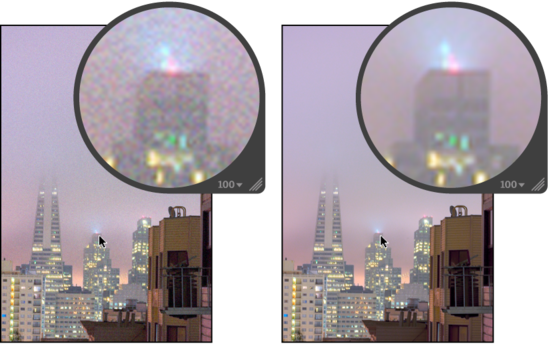
\includegraphics[width=15cm]{szum}
		\caption{Przed i po operacji odszumiania fotografii}
		Źródło: http://fotografiaparaprincipianntes.blogspot.com/2014/02/nitidez-vs-reduccion-de-ruido-en-lr.html (dostęp z dn. 01.05.2021)
	\end{figure}
	\par
	Ważnym procesem przy ustalaniu przez maszynę elementów planu pierwszego, \linebreak drugiego i tak dalej jest binaryzacja. Polega ona na zapisaniu każdego piksela fotografii zero-jedynkowo. Zero odpowiada barwie białej a jeden analogicznie barwie czarnej. Po co maszynie wiedza co jest tłem a co nie? W moim projekcie wykorzystuję binaryzację obrazu przechwyconego z kamery komputerowej do detekcji człowieka i tła. Istotnym elementem jest kolorystyka trzymanego w dłoni obiektu i analiza jej barwy przez odpowiednie funkcje. Komputer w ten sposób potrafi rozpoznać barwę i odseparować obiekt w kolorze od reszty tła. Warunkiem jest brak barwy interesującego nas obiektu w palecie barw tła - w innym wypadku algorytm może obrać za cel niewłaściwy element otoczenia. Wracając do procesu binaryzacji, sekret tkwi w ustaleniu granicy kiedy dany piksel ma być zerem a kiedy jedynką. Pomaga nam w tym zabieg zwany progowaniem (z angielskiego thresholding). Jego zdaniem jest wyznaczenie pewnego progu jasności i podzielenie pikseli na zera (jeżeli mniejsze od tej wartości) i jedynki (jeżeli większe). Poniżej porównanie fotografii oryginalnej (po prawej) i fotografia poddana procesowi binaryzacji:
	\begin{figure}
		\centering
		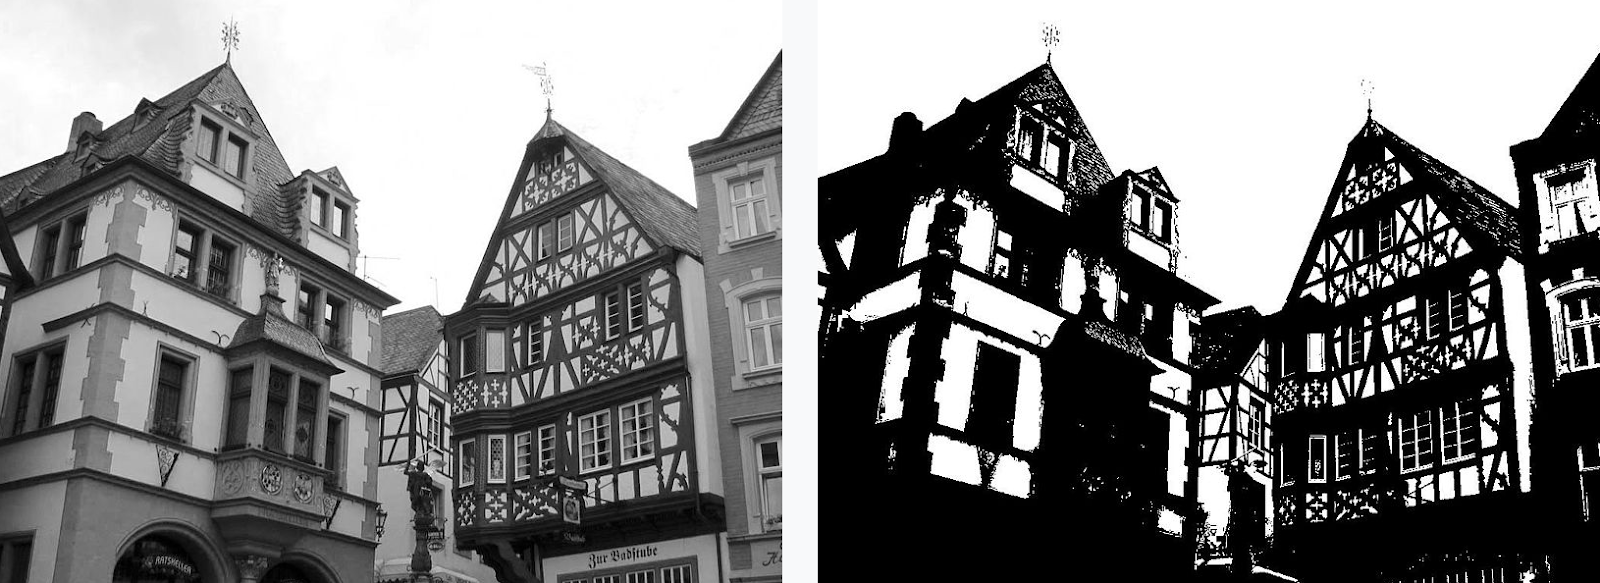
\includegraphics[width=15cm]{binary}
		\caption{Przed i po operacji binaryzacji fotografii}
		Źródło: https://en.wikipedia.org/wiki/Otsu\%27s\_method (dostęp z dn. 24.04.2021)
	\end{figure}
	\subsection{Rozpoznawanie twarzy}
	\par
	Algorytmy rozpoznawania twarzy są z nami od tysięcy lat. Przez te wszystkie lata działy się one w naszej głowie i to domeną ludzi było analizowanie i porównywanie twarzy ludzi. Stosunkowo niedawno jednak naukowcy zaczęli rozwijać podobne algorytmy u maszyn. Zacznijmy od początku. Według amerykańskiego naukowca i filozofa zajmującego się naukami poznawczymi Jerry'ego Fodora\cite{ref15} umysł ludzki ma strukturę modularną. Koncepcja modularności umysłu mówi o dwóch warstwach, na jakie podzielony jest nasz umysł:
	\begin{itemize}
		\item Centralną
		\item Modularną
	\end{itemize}
	\par
	Aby wyjaśnić jak działa centralna część naszego umysłu trzeba odpowiedzieć sobie na pytanie, w który miejscu naszego mózgu rodzą się emocje? Czym one są i jaki mają wpływ na działanie pozostałych części naszego mózgu? Z biologicznego punktu widzenia emocje są związane z funkcjonowaniem układu limbicznego. Z fizjologicznego punktu podejścia są uważane za bardzo złożone reakcje automatyczne, a także za wynik rozszerzania mechanizmów procesu zachodzącego w mózgu jakim jest homeostaza. Homeostaza jest procesem odpowiedzialnym za równowagę całego organizmu, w którym zachodzi niezliczona liczba reakcji neuropsychologicznych. Podwzgórzem nazywamy miejsce, gdzie ma miejsce transmisja impulsów neurologicznych na sygnały biochemiczne. Innymi słowy to tutaj układ nerwowy jest połączony z układem hormonalnym naszego organizmu. Wracając do centralnej części naszego umysłu, według Fodora, jest ona odpowiedzialna za kreatywną i emocjonalną część ludzkiej egzystencji. To właśnie ta część jest ściśle powiązana z naszą świadomością i jest odpowiedzialna za przetwarzanie danych zanim te dotrą do narządów odpowiedzialnych za pięć zmysłów takich jak dotyk, węch, smak, wzrok i słuch. W momencie, w którym człowiek ma uszkodzone te części mózgu odpowiedzialne za przekazywanie wyżej wymienionych sygnałów neurologicznych nie jest on w stanie na poprawne zinterpretowanie konkretnych rzeczy (czyli sygnałów płynących ze świata zewnętrznego). Na przykład nie jest w stanie ocenić czy jabłko, na które patrzy jest elementem żywym czy martwym. Zaburzone jest postrzeganie świata i rozumienie elementarnych podstaw, które są wpisane w naturalną egzystencję człowieka. Na podobnej zasadzie działają interfejsy programowania aplikacji (API), które odciążają programistów od analizy jak działa program a tym co powinien robić. Tym samym człowiek odpowiedzialny za obsługę takiego API nie ma obowiązku posiadania wiedzy na temat szczegółowych operacji zachodzących po drugiej stronie systemu. Interesuje go tylko jakie dane musi dostarczyć  interfejsowi na wejściu i co powinien otrzymać na wyjściu.
	\par
	Z pomocą przyszły sieci neuronowe i sztuczna inteligencja, które w ostatniej dekadzie zyskały bardzo szeroki rozgłos w szeroko pojętej dziedzinie Information-Technology. Co to dokładnie jest i na czym polega? Żeby to zrozumieć trzeba rozbić widzenie na czynniki pierwsze. Posłużę się analogią przy procesie rozpoznawania ludzkiej twarzy. Nasz zmysł wzroku skupia się na istotnych szczegółach, na które składają się elementy naszej twarzy takie jak uszy, nos, oczy, usta, rozstaw i odstępy pomiędzy poszczególnymi elementami. To dopiero wstęp do biometrii. Cyfrowe przedstawienie twarzy można opisać za pomocą cech biometrycznych człowieka. Te z kolei grupują się na dwa obozy: cechy geometryczne i antropometryczne.
	\begin{enumerate}
		\item Cechy geometryczne:
		\begin{enumerate}
			\item Kształt twarzy
			\item Szerokość twarzy
			\item Kształt ust
			\item Kształt nosa
			\item Kształt czoła
			\item Kształt brwi
			\item Kształt podbródka
			\item Kształt uszu
		\end{enumerate}
		\item Cechy antropometryczne:
		\begin{enumerate}
			\item Rozstaw oczodołów
			\item Odległość między kącikami oczu
			\item Dystans między oczami a nosem
			\item Dystans między linią oczu a linią ust
		\end{enumerate}
	\end{enumerate}
	\begin{figure}
		\centering
		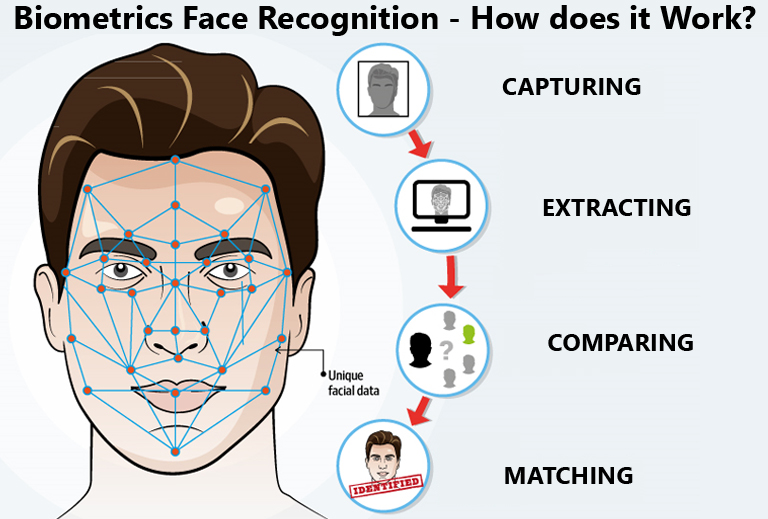
\includegraphics[width=15cm]{face}
		\caption{Cechy ludzkiej twarzy, źródło}
		Źródło: https://www.starlinkindia.com/blog/biometrics-face-recognition/ (dostęp z dn. 06.05.2021)
	\end{figure}
	\par
	Metoda rozpoznawania twarzy podzielona jest na trzy składowe, których wynikiem jest rozpoznanie lub jego brak przez ten algorytm. Pierwszą składową jest fizyczne zestawienie kształtów z kolorami i analiza obrazu pod kątem kontrastu, jasności, cieni i gradientów występujących na twarzy. Następnie obiektyw kamery porównuje współrzędne powyższych elementów i analizuje paletę barw w tych miejscach (osoby z dużym nosem będą miały inny współrzędne końca cienia rzucanego przez tę część ciała). Proces ten zalicza się do kategorii strukturalnych. Ostatnią składową jest porównanie matematyczne. Algorytm porównuje przekształcenia obrazu i na tej podstawie potrafi ocenić czy wcześniejsze wyliczenia mają swoje odzwierciedlenie dla wspomnianych transformacji obrazu. Przekształcenia obrazów dzielimy na pięć kategorii:
	\begin{itemize}
		\item Przekształcenia geometryczne
		\item Przekształcenia punktowe
		\item Przekształcenia kontekstowe
		\item Przekształcenia widmowe
		\item Przekształcenia morfologiczne	
	\end{itemize}
	\subsection{Przekształcenia obrazów}
	\par
	Nierzadko stosuje się zabiegi przekształceń celem przygotowania danych wejściowych dla pewnego systemu, który mógłby błędnie zinterpretować przesunięcia, rotacje czy przybliżenia, które dla człowieka nie stanowiłyby problemu, ale dla komputera już tak. Tak przygotowane dane są “bardziej czytelne” dla oprogramowania, którym zadaniem jest przetworzenie obrazu i potencjalna analiza obiektów się na nim znajdujących.
	\par
	Przekształcenia geometryczne uzyskuje się z pomocą przekształceń afinicznych, które polegają na mnożeniu macierzy obrazu z jej współrzędnymi i nie tylko. Przykładowa macierz:
	\[
	\begin{bmatrix}
		x\\
		y
	\end{bmatrix}
	=
	\begin{bmatrix}
		z_{00} & z_{01} & z_{02}\\
		z_{10} & z_{11} & z_{12}
	\end{bmatrix}
	\begin{bmatrix}
		x'\\
		y'\\
		1
	\end{bmatrix}
	\]
	\par
	Translacja to inaczej przesunięcie układu współrzędnych względem jego \linebreak początkowych wartości. Pierwszy z brzegu przykład macierzy, która przekształca żądany obraz o a jednostek (pikseli) na osi x oraz b jednostek (pikseli) na osi y, wygląda następująco:
	\[
	\begin{bmatrix}
		x\\
		y
	\end{bmatrix}
	=
	\begin{bmatrix}
		1 & 0 & a\\
		0 & 1 & b
	\end{bmatrix}
	\begin{bmatrix}
		x'\\
		y'\\
		1
	\end{bmatrix}
	\]
	Przyrównując a do czterdziestu i b do osiemdziesięciu otrzymujemy następujące przekształcenie:
	\begin{figure}
		\centering
		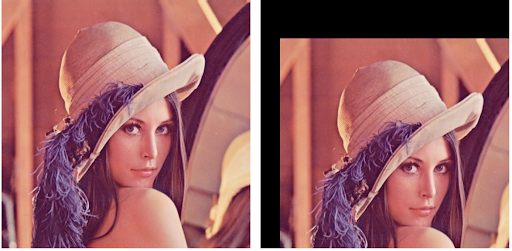
\includegraphics[width=15cm]{translation}
		\caption{Translacja obrazu}
		Źródło: http://analizaobrazu.x25.pl/articles/23 (dostęp z dn. 09.05.2021)
	\end{figure}
	\par
	Skalowanie obrazu czy manipulacja perspektywą w układzie współrzędnych z osiami x, y, z ma za zadanie przybliżyć bądź oddalić od widza obraz, na który ów widz patrzy. Przykładowa macierz:
	\[
	\begin{bmatrix}
		x\\
		y
	\end{bmatrix}
	=
	\begin{bmatrix}
		a & 0 & 0\\
		0 & b & 0
	\end{bmatrix}
	\begin{bmatrix}
		x'\\
		y'\\
		1
	\end{bmatrix}
	\]
	\par
	Zmienne a i b odpowiadają kolejno za “rozciąganie” obrazu w poziomie i pionie. Jeżeli chcemy przeskalować obraz w poziomie o wartość 0.5, a w pionie o 1.5 to wyniki przedstawione są poniżej:
	\begin{figure}
		\centering
		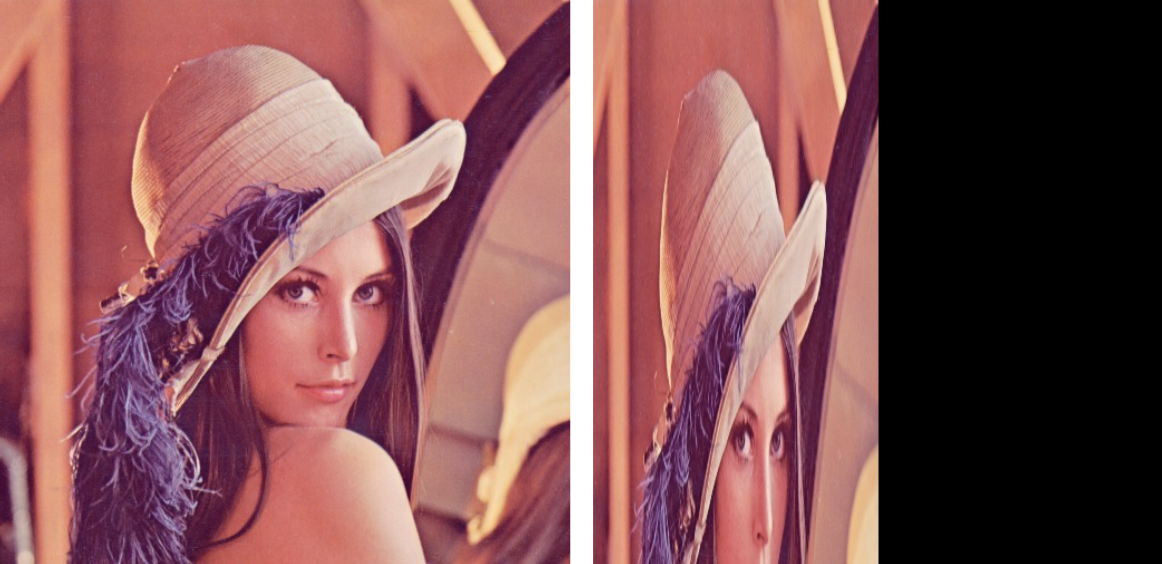
\includegraphics[width=15cm]{scale}
		\caption{Skalowanie obrazu}
		Źródło: http://analizaobrazu.x25.pl/articles/23 (dostęp z dn. 09.05.2021)
	\end{figure}
	\par
	Istnieją jeszcze przekształcenia, które mają na celu obroty, pochylenie czy przekształcenie panoramiczne obrazu. Ten ostatni przykład jest ciekawy w kontekście przygotowania obrazu do analizy dla maszyny, o czym już wspomniałem nieco wyżej. Nałożenie na obraz kilku przekształceń ustawia nam (a bardziej oprogramowaniu do analizy) obraz z układem współrzędnych w dwuwymiarowej warstwie. Ignoruje ona oś z i można powiedzieć, że nagina pozostałe dwie osie, aby obiekty zawarte na obrazie można było opisać przy pomocy współrzędnych układu dwuwymiarowego. Przykładem zastosowania takiego rozwiązania możemy być detekcja i analiza samochodowych tablic rejestracyjnych. Nie zawsze bywa, że auto jest ustawione idealnie na wprost do obiektywu kamery i maszyna musi dokonać przekształcenia panoramicznego, aby odczytać litery i cyfry. Pamiętajmy, że algorytmy muszą dosyć sprawnie poradzić sobie z tym zadaniem w ciągu maksymalnie kilku sekund od rozpoczęcia analizy. Wykorzystuje się do tego na przykład bibliotekę OpenCV, o której już pisałem. Poniżej przedstawienie przykładu przekształcenia panoramicznego:
	\begin{figure}
		\centering
		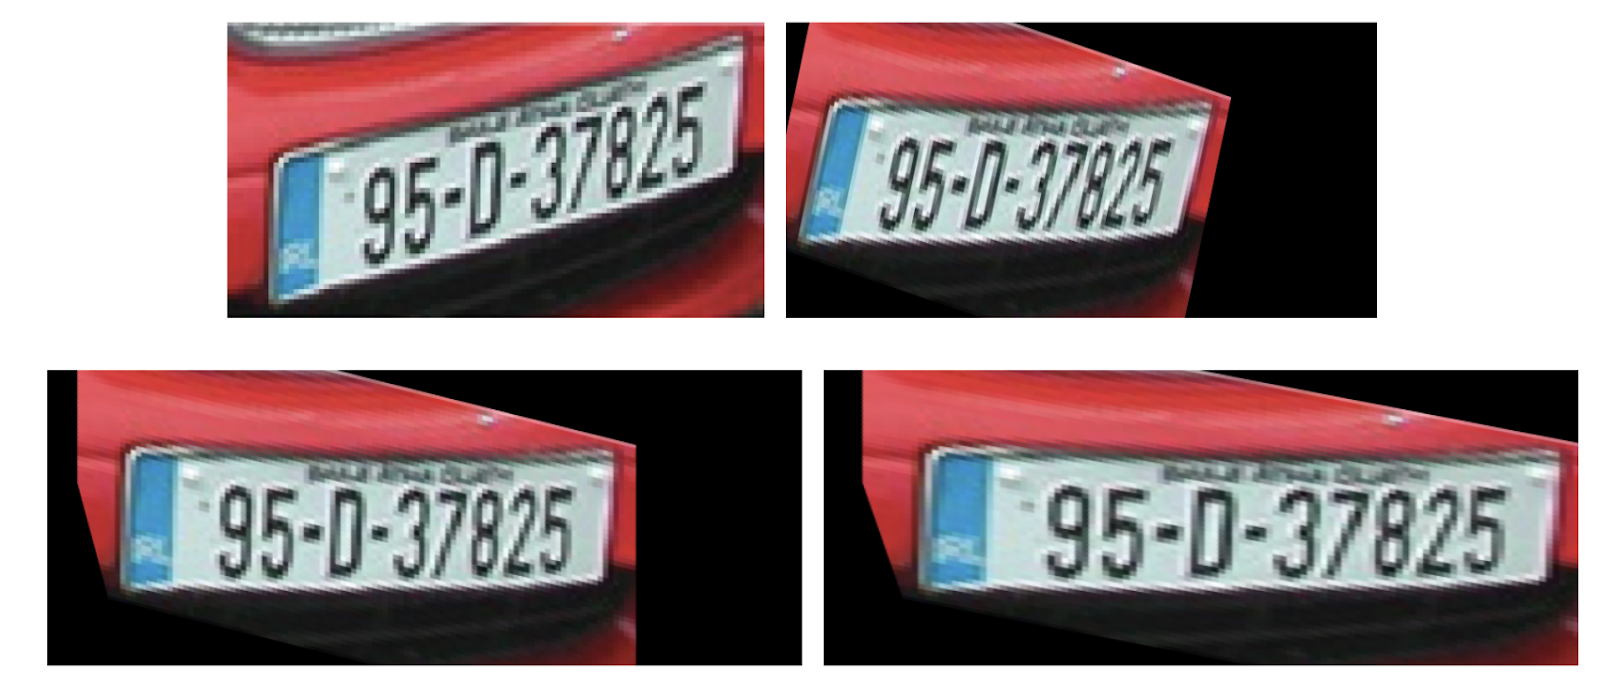
\includegraphics[width=15cm]{plates}
		\caption{Transformacja tablic rejestracyjnych}
		Źródło: http://analizaobrazu.x25.pl/articles/23 (dostęp z dn. 09.05.2021)
	\end{figure}
	\par
	Tak przygotowany obraz nie jest jeszcze gotowy i wymaga poddania go na przykład procesu binaryzacji czyli wyeliminowanie drugiego planu i wyselekcjonowanie obiektów znajdujących się na pierwszym planie. Warto zwrócić uwagę, że pomoca jest paleta barw, która jest zawarta w większości tablic rejestracyjnych (W Wielkiej Brytanii, Holandii lub Luksemburgu zamiast białego stosuje się złoty kolor, który równie dobrze kontrastuje z czernią).
	\subsection{Rozpoznawanie obiektów}
	\par
	Pisząc o rozpoznawaniu obiektów będę zawężał swoje rozważania do detekcji obiektów w materiale wideo. Jak wiemy, film składa się z sekwencji klatek, które są analizowane przez oprogramowania do rozpoznawania obiektów. Na początku komputerowi należy określić zbiór bądź grupę elementów, które w konkretnym zestawieniu w określonej odległości będą znaczyły o pojawieniu się w obiektywie kamery żądanego obiektu. Może to być na przykład twarz ludzka, a systemy, które wykorzystują takie algorytmy są szeroko stosowane w monitoringu publicznym we wschodniej Azji (między innymi w Chinach, Japonii, Korei czy SIngapurze). Mimo, że prężnie rozwijający się sektor gospodarki odpowiedzialny za nowoczesne technologie z dziedziny cyfrowej analizy obrazów znajduje się w wyżej wymienionych krajach to jest jeden kraj w Europie, który pod względem inwigilacji publicznej nie ma sobie równych. Wielka Brytania, bo o niej mowa, posiada według statystyk z 2016 roku największą ilość kamer włączając w to kamery na przystankach autobusowych, ale też na prywatnych posesjach.
	\begin{figure}
		\centering
		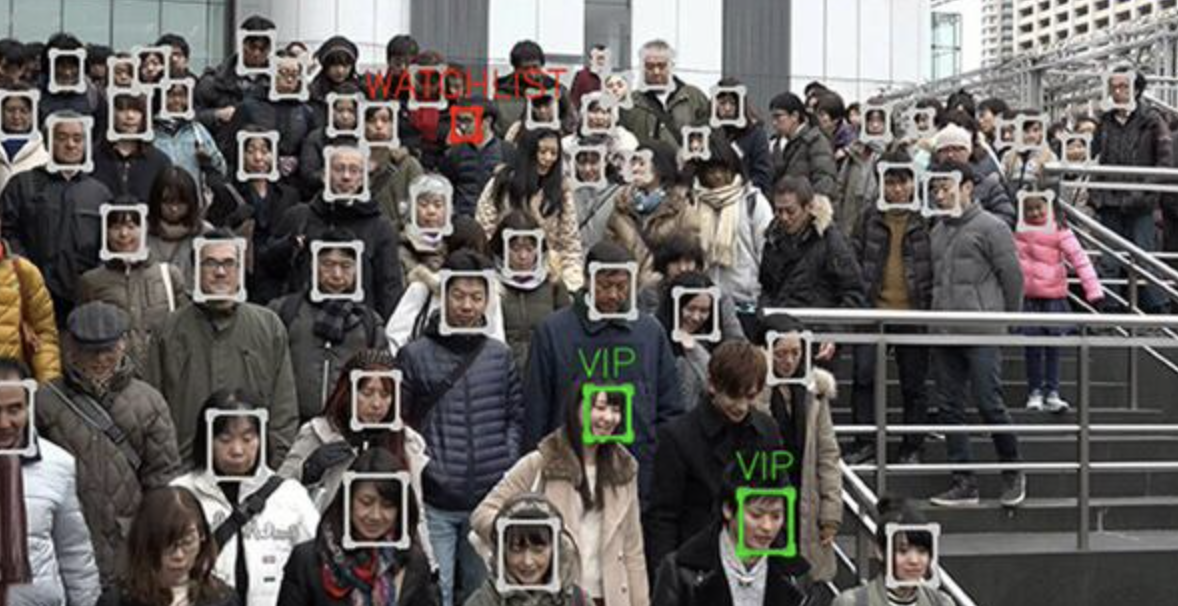
\includegraphics[width=15cm]{detect}
		\caption{Ujęcie kamery publicznego monitoringu w Azji}
		Źródło: https://www.eetasia.com/the-current-reality-of-facial-recognition/ (dostęp z dn. 26.04.2021)
	\end{figure}
	\par
	Powyżej przykład ujęcia z kampanii reklamowej korporacji zajmującej się sektorem publicznego monitoringu. Widać tutaj dokładność z jaką “oko” kamery jest w stanie dostrzec i prawidłowo ocenić wymiary oraz odległość ludzkiej twarzy. Nierzadko się zdarza, że dodatkowy zestaw danych, o których wspomniałem, ma za zadanie zidentyfikować konkretny typ urody, przykładowo tylko osoby o ciemniejszej karnacji i ciemnymi włosami. Organy ścigania wykorzystują podobne sposoby do “wyłapywania” z tłumu ludzi poszukiwanych listem gończym.
	\par
	Rozpoznawanie twarzy to jeden z wielu przykładów wykorzystania algorytmów do przeszukiwania konkretnych obiektów. Znane są również algorytmy zaimplementowane w komputer pokładowy nowoczesnych samochodów z detekcją przekroczenia linii bocznej lub z asystą automatycznego parkowania. Za wszystkim stoi uczenie maszynowe z wykorzystaniem sieci neuronowych. Dzisiejsze możliwości w kontekście mocy obliczeniowej maszyn pozwalają na tworzenie bardzo skomplikowanych operacji na zadanym zbiorze testowym w celu systematycznej nauki i poszerzania swojej “wiedzy”, aby sprawniej eliminować niepoprawne przypadki i dokładniej identyfikować elementy na zdjęciu.
	
	\section{Projekt interaktywnej kolorowanki wykorzystującą cyfrową \linebreak analizę obrazu z wykorzystaniem sztucznej inteligencji}
	
	\subsection{Kod aplikacji}
	
	\begin{lstlisting}[language=C++, caption=Początek wywołania. Źródło: Własne]
		VideoCapture cap(0);
		
		//sprawdzenie dostepu do kamery urzadzenia
		if ( !cap.isOpened() )
		{
			cout << "Cannot open the web cam" << endl;
			return -1;
		}
		
		//uruchomienie okna z przechwyconym obrazem z kamery
		namedWindow("Control", WINDOW_AUTOSIZE);
	\end{lstlisting}
	
	Powyższy fragment kodu jest pierwszymi linijkami głównej metody wywołującej o nazwie main. Na początku sprawdzam czy mamy dostęp do kamery urządzenia. Następnie tworzę okno o automatycznych rozmiarach (skalowane w zależności od ustawień komputera, na którym uruchamiany jest kod).
	
	\newpage
	
	\begin{lstlisting}[language=C++, caption=Klawisze funkcyjne. Źródło: Własne]
		if (dArea > 10000) {
			int posX = dM10 / dArea;
			int posY = dM01 / dArea;        
			
			if (iLastX >= 0 && iLastY >= 0 && posX >= 0 && posY >= 0) {
				if (waitKey(60) == 113) {
					line(imgLines, Point(posX, posY), Point(iLastX, iLastY), Scalar(0,0,255), 15);
				}
				if (waitKey(60) == 119) {
					line(imgLines, Point(posX, posY), Point(iLastX, iLastY), Scalar(0,255,0), 15); 
				}
				else if (waitKey(60) == 101)
				{
					line(imgLines, Point(posX, posY), Point(iLastX, iLastY), Scalar(0,0,0), 15); 
				}
			}
			iLastX = posX;
			iLastY = posY;
		}
	\end{lstlisting}

	\newpage
	
	Powyżej zaimplementowane jest reagowanie programu na naciśnięte klawisze klawiatury komputera. Każdy przycisk zakodowany jest w formacie liczbowej i ma swoje odzwierciedlenie w tablicy znaków ASCII
	
	\begin{figure}
		\centering
		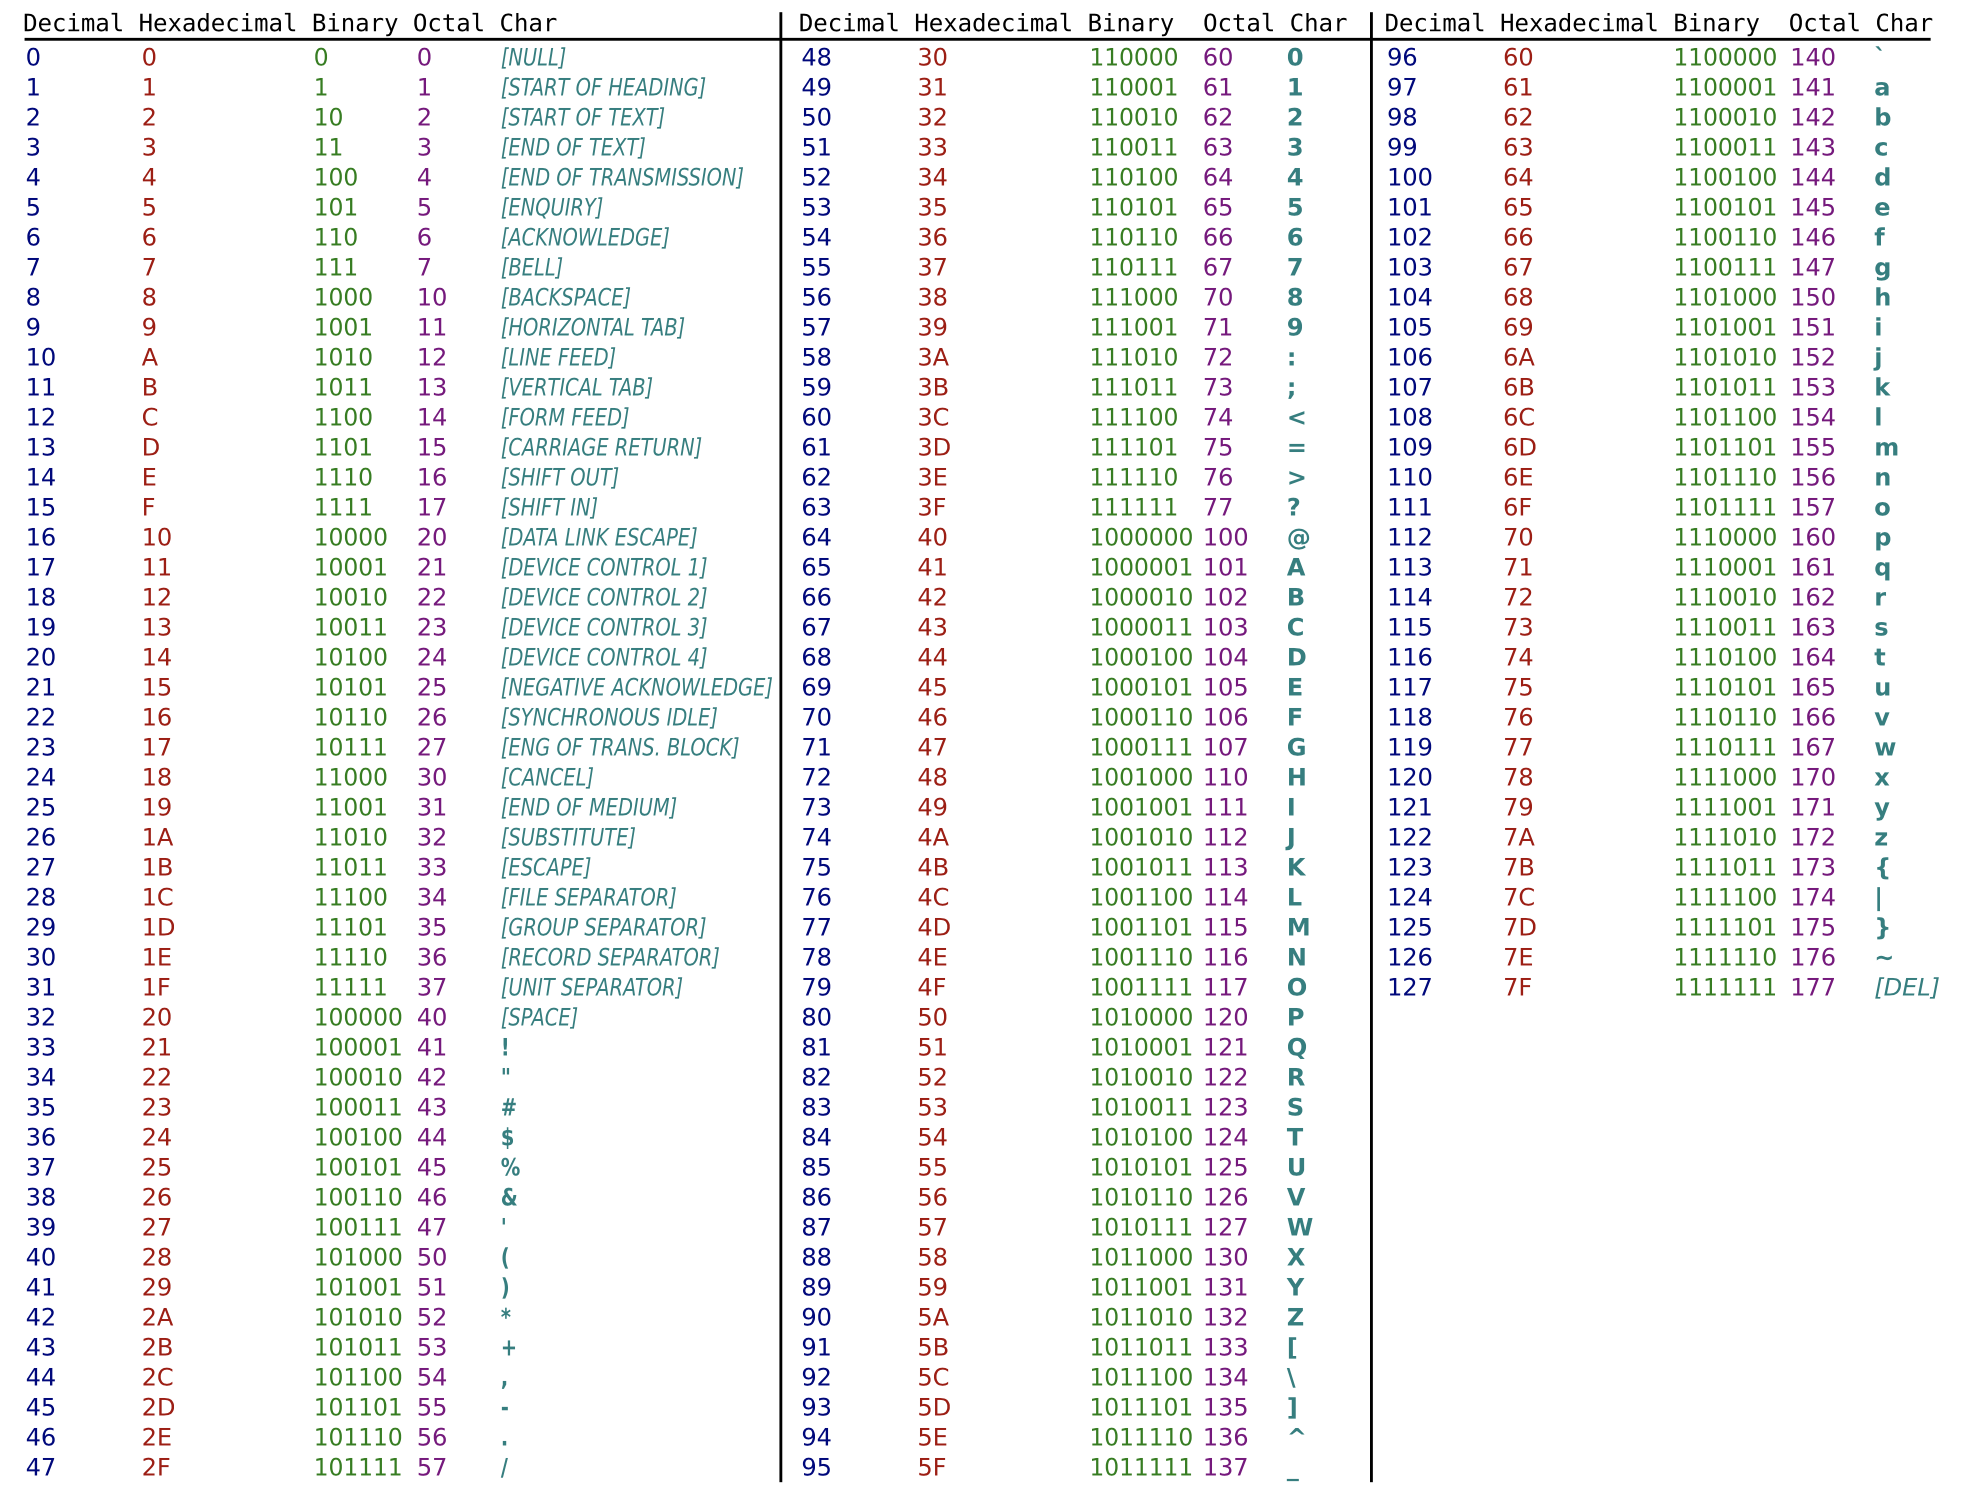
\includegraphics[width=15cm]{ascii}
		\caption{Tablica znaków ASCII}
		Źródło: https://commons.wikimedia.org/wiki/File:ASCII-Table.svg (dostęp z dn. 19.11.2020)
	\end{figure}
	
	\newpage
	
	\section*{\textbf{Fragmenty kodu oprogramowania z wyjaśnieniami} }
	
	\begin{lstlisting}[language=C++, caption=Nakładanie obrazu do kolorowania. Źródło: Własne]
		//Funkcja odpowiedzialna za nalozenie na plotno zadanego obrazu
		void overlayImage(const cv::Mat &background, const cv::Mat &foreground, 
		cv::Mat &output, cv::Point2i location)
		{
			background.copyTo(output);
			for(int y = std::max(location.y , 0); y < background.rows; ++y)
			{
				int fY = y - location.y;
				if(fY >= foreground.rows)
				break;
				for(int x = std::max(location.x, 0); x < background.cols; ++x)
				{
					int fX = x - location.x;
					if(fX >= foreground.cols)
					break;
					double opacity =
					((double)foreground.data[fY * foreground.step + fX * foreground.channels() + 3])
					
					/ 255.;
					for(int c = 0; opacity > 0 && c < output.channels(); ++c)
					{
						unsigned char foregroundPx =
						foreground.data[fY * foreground.step + fX * foreground.channels() + c];
						unsigned char backgroundPx =
						background.data[y * background.step + x * background.channels() + c];
						output.data[y*output.step + output.channels()*x + c] =
						backgroundPx * (1.-opacity) + foregroundPx * opacity;
					}
				}
			}
		}
	\end{lstlisting}
	
	Funkcja overlayImage z argumentami: background, foreground, output i location jest odpo- wiedzialna za nałożenie na przechwycony obraz z kamery durgiej warstwy - w tym wypadku jest to fragment obrazka do pokolorowania (same kontury).
	Funkcja w linijce szóstej rozpoczy- na pętle, której zadaniem jest w osiach x i y przychodzących macierzy background i foreground obliczenie i ustawienie w środku generowanego okna obrazu. W linijce 11 zaczyna się sprawdzenie dla osi x po uprzedmim sprawdzeniu osi y. Następnie po ustawniu punktów lokalizacyjnych, w linijce 20 nanoszone są zmiany na ekran poprzez przypisanie mapie nazwie data, która jest elementem zarowno macierzy background jak i foreground.
	\newpage
	\subsection{Cel badania}
	\par
	Moim nadrzędnym celem badania było potwierdzenie tezy, o której wspominałem we wstępie niniejszej pracy. Jako, że w mojej rodzinie posiadam wielu nauczycieli edukacji wczesnoszkolnej postanowiłem wykorzystać ten fakt i skorzystać z pomocy podopiecznych moich bliskich. Za cel obrałem dzieci w wieku od trzech do pięciu lat oraz podzieliłem porówno na chłopców i dziewczynki. Selekcję płciową zastosowałem w celu dodatkowego potwierdzenia tezy, że dziewczynki w tym wieku są bardziej zaciekawione i zaangażowane w zajęcia dydaktyczne prowadzone przez nauczyciela.
	
\begin{table}[h!]
	\centering
	\begin{tabular}{|c|c|c|c|c|c|c|}
		\hline
		\multicolumn{1}{|l|}{Lp.} & \multicolumn{1}{l|}{Wiek} & \multicolumn{1}{l|}{Płeć}  \\ \hline
		Dziecko 1.                & 3                              & Dziewczynka                                          \\ \hline
		Dziecko 2.                & 4                              & Chłopiec                                       \\ \hline
		Dziecko 3.                & 3                              & Chłopiec                                              \\ \hline
		Dziecko 4.                & 5                              & Dziewczynka                                          \\ \hline
		Dziecko 5.                & 4                              & Dziewczynka                                            \\ \hline
		Dziecko 6.                & 5                              & Dziewczynka                                               \\ \hline
	\end{tabular}
	\caption{Dane dzieci biorących udział w badaniu}
	Źródło: Własne
\end{table}
	
	\par
	Ze względu na to, że czas skupienia małych dzieci jest proporcjonalny do ich wieku uznałem, że na każdego badanego poświęcę nie więcej niż minutę. Każde dziecko otrzymało niebieski klocek, który służył jako marker dla obiektywu kamery. Do obsługi programu wymagana jest umiejętność wciskania dwóch klawiszy. Mimo, że program posiada dodatkowe funkcje takie jak usuwanie zamalowanego obszaru (gumka to potężne narzędzia dla małego dziecka) nie zdecydowałem się na przeprowadzenie dodatkowych obserwacji dzieci przy manipulacji ustawień oprogramowania. W ogóle o nich nie wspomnialem nie chcąc, aby zapomniały o początkowych ustaleniach celu badania - pokolorowaniu jabłka na czerwono i zielono według wyświetalnego konturu. Dobór niebieskiego klocka nie jest przypadkowy. Aplikacja została tak zaprogramowana, aby śledzić konkretny pigment i kolorować płótno po naciśnięciu odpowiedniego klawisza.
	
	
	\subsection{Opis badania}
	
\par Badanie zgodnie z planem trwało nie więcej niż minutę na każde dziecko. Gdyby jednak stało się tak, że wyszłoby poza ustalone ramy czasowe badanie mogłoby uzyskać niewspółmierne wyniki. Dlaczego? Dzieci zaczęły zapominać o początkowych ustaleniach i rysowały różne przedmioty nieskupiając się na pokolorowaniu jabłka - wnioskuję to po ogólnym rozsierdzeniu i rozkojarzeniu większości badanych po upływie niespełna minuty. Niemniej jednak większość dzieci wykonało zadanie, choć warunki nie były idealne. Oprogramowanie jest zależne od natężenia światła w pomieszczeniu, kolorów, które wyłapuje kamera (w przedszkolu kamera oszalała dlatego wybrałem pobieloną ścianę w jednej z sal). Dodatkowo detekcja jest bardzo wyczulona na odcienie niebieskiego. Na szczęscie takich niechcianych zdarzeń nie zaobserwowałem choć mój scenariusz badania brał taką ewentualność pod uwagę. Na początku badania poświęcałem góra dziesięć sekund na szybkie i zrozumiałe wytłumaczenie działania kolorowanki. Ku mojemu zaskoczeniu prawie każde dziecko nie wymagało szczególnych wskazówek. Łapały wszystko w lot i chętnie współpracowały. Ich aktywność była nadwyraz zaskakująca, nawet dla nauczyciela, który czuwał obok przez czas trwania badania. Zdarzały się sytuacje, w których oprogramowanie nie potrafiło dokładnie oszacować szukanego kolory, ale ponowne uruchomienie aplikacji i zmiana kąta nachylenia laptopa pozwalał na pozbycie się tego problemu.
	\par Badanie polegało na jednoczesnym wciśnięciu klawisza odpowiedzialnego za kolor czerwony lub zielony. Następnie w miejscu, w którym kamera komputera zlokalizowała niebieski korek trzymany przez dziecko, program po wciśnięciu odpowiedniego klawisza malował w tym miejscu linię o barwie odpowiadającej wciśniętemu klawiszowi. Na ekranie komputera wyświetlał się biały kontru jabłka z wyraźną obramówką owocu z listkiem w jego górnej części. Badanie kończyło się po upływie niespelna minuty lub w momencie, w którym dziecko osiągnęło cel badania - pokolorowało jabłko.
	
\subsection{Wyniki badania}
	
\par Zgodnie z oczekiwaniami część dzieci traciła zainteresowanie po upływie pół minuty, ale pozostali wzorowo wykonali zadanie. Choć funkcjonalność zmiany koloru była punktem, w którym większość badanych nie potrafiła się odnaleźć, tak prawie w każdym przypadku dziecko wiedziało kiedy należy zmienić kolor, bo owoc został już pomalowany na czerwono. Zdarzały się pojedyncze przypadki, w których pierwszym kolorem był odcień zielonego. Dlaczego? Być może wynika to z psychologii dziecka, które chcąc zacząć od z pozoru prostszych i mniejszych rzeczy może w przyszłości być osobą niepewną w swoich działaniach i niewierzącą w swoje umiejętności. Mimo kilku błędów oprogramowania, częściowym braku zaangażowania niektórych dzieci oraz ogólnej destabilizacji uwagi badanego dziecka w kluczowych momentach badania uważam badanie za udane. Ponad połowa dzieci wykonała zadanie, co pozwoliło zebrać wyniki, opisać je i porównać, a następnie wyciągnąć wnioski.
	

\begin{figure}[bp!]
	\centering
	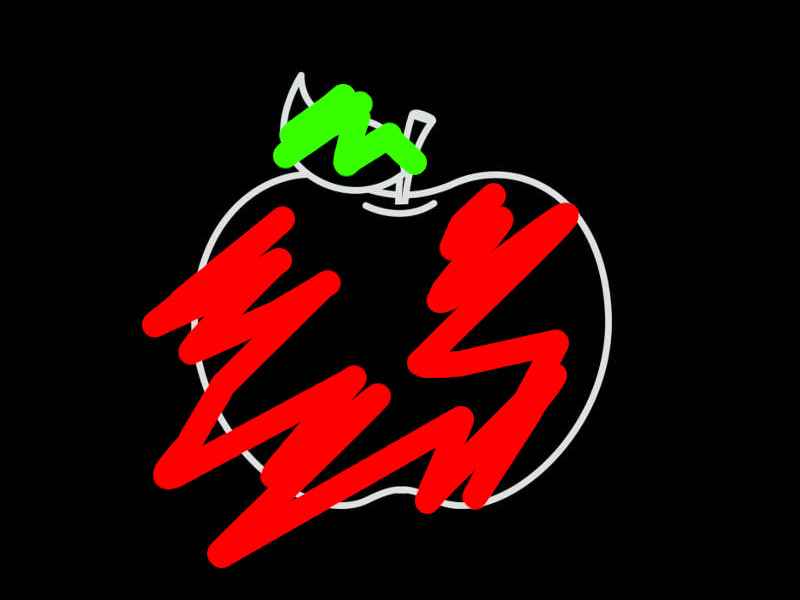
\includegraphics[width=10cm]{wyniki/1}
	\caption{Wynik 1. badania}
	Źródło: Własne
\end{figure}

\begin{figure}[bp!]
	\centering
	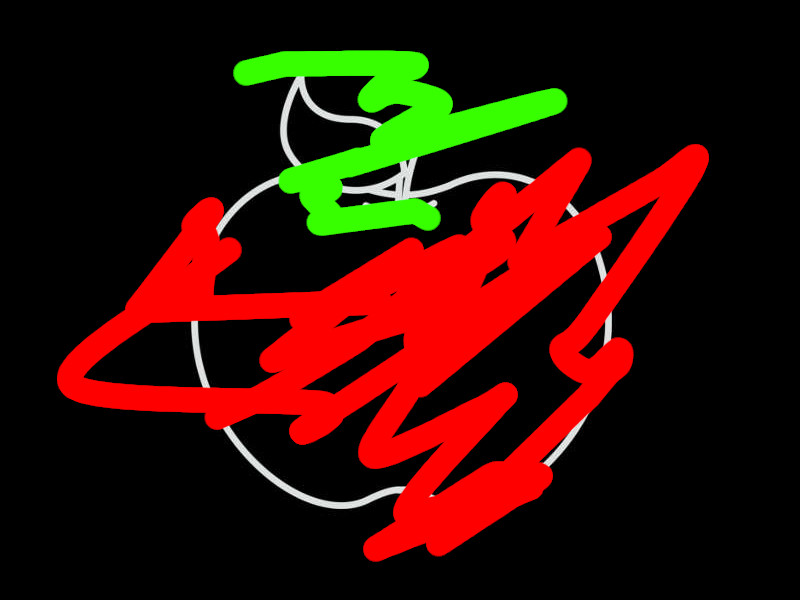
\includegraphics[width=10cm]{wyniki/2}
	\caption{Wynik 2. badania}
	Źródło: Własne
\end{figure}

\begin{figure}[bp!]
	\centering
	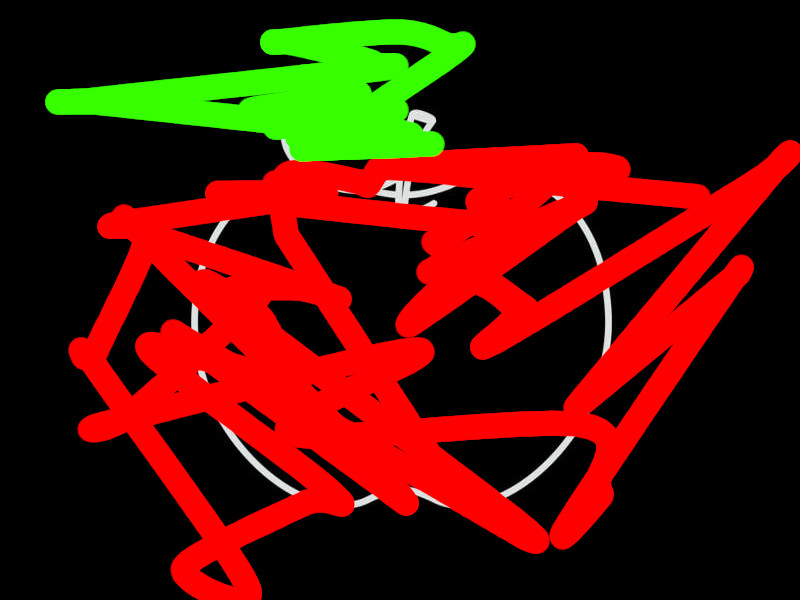
\includegraphics[width=10cm]{wyniki/3}
	\caption{Wynik 3. badania}
	Źródło: Własne
\end{figure}

\begin{figure}[bp!]
	\centering
	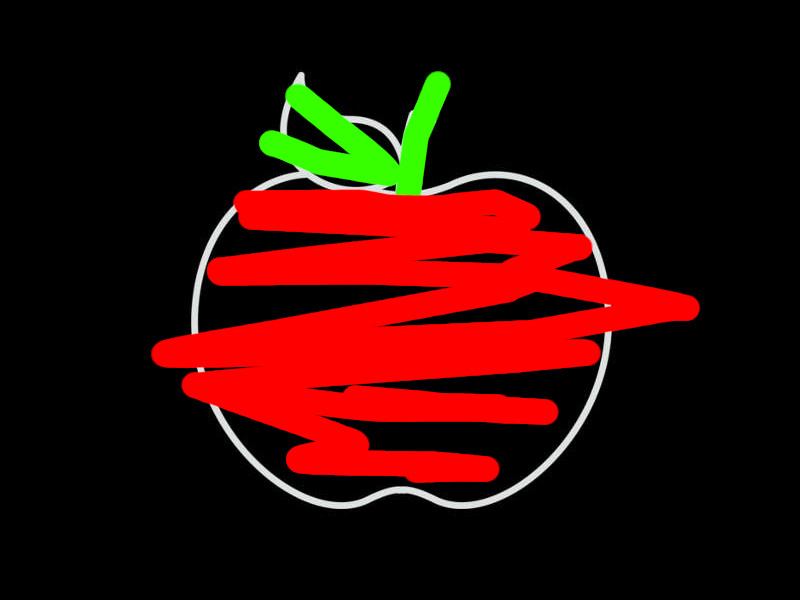
\includegraphics[width=10cm]{wyniki/4}
	\caption{Wynik 4. badania}
	Źródło: Własne
\end{figure}

\begin{figure}[bp!]
	\centering
	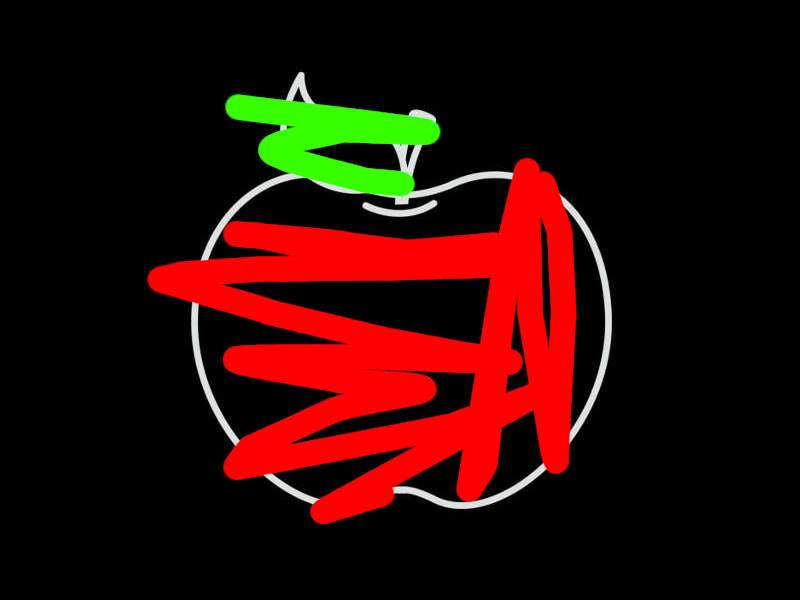
\includegraphics[width=10cm]{wyniki/5}
	\caption{Wynik 5. badania}
	Źródło: Własne
\end{figure}

\begin{figure}[bp!]
	\centering
	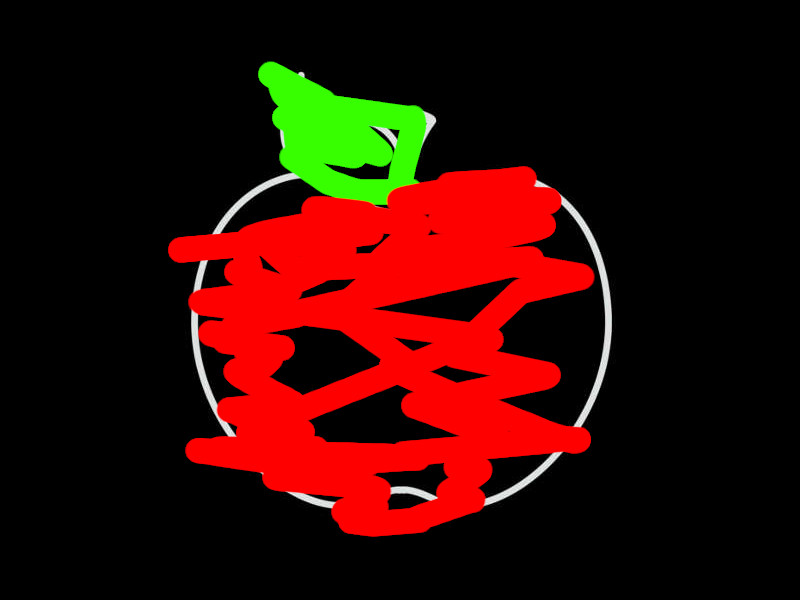
\includegraphics[width=10cm]{wyniki/6}
	\caption{Wynik 6. badania}
	Źródło: Własne
\end{figure}

\par Jak widać na powyższych wynikach każde dziecko ze stuprocentową pewnością potrafiło zadecydować co powinno być czerwone a co zielone. Potrafiły poprawnie zlokalizować elementy na rysunku, nazwać je i przypisać odpowiedni kolor. Na ten moment wszystko było zgodnie z początkowymi założeniami badania. Na niektórych obrazkach da się zauważyć rozpoczęcie malowania w kierunku wertykalnym lub horyzontalnym. Nierzadko zdarzały się chaotyczne ruchy ręką co utrudniało zlokalizowanie białego konturu jabłka. Ponad połowa zamalowanej powierzchni stanowiło powierzchnie jabłka. Część dzieci rysowała podlużnymi ruchami ręki, a część krótkimi ale liczniejszymi ruchami.


	\begin{table}[]
	\centering
	\begin{tabular}{|c|c|c|c|c|c|c|}
		\hline
		\multicolumn{1}{|l|}{Lp.} & \multicolumn{1}{l|}{Rozpoznanie} & \multicolumn{1}{l|}{1. Kolor} & \multicolumn{1}{l|}{Ruchy} & \multicolumn{1}{l|}{\% zamalowania} & \multicolumn{1}{l|}{\% poza} & \multicolumn{1}{l|}{czas (s)} \\ \hline
		Dziecko 1.                & TAK                              & Czerwony                      & Wertykalne                 & 65                                  & 5                            & 34                            \\ \hline
		Dziecko 2.                & TAK                              & Czerwony                      & Chaotyczne                 & 80                                  & 10                           & 47                            \\ \hline
		Dziecko 3.                & TAK                              & Czerwony                      & Chaotyczne                 & 85                                  & 20                           & 52                            \\ \hline
		Dziecko 4.                & TAK                              & Zielony                       & Horyzontalne               & 90                                  & 5                            & 56                            \\ \hline
		Dziecko 5.                & TAK                              & Czerwony                      & Horyzontalne               & 85                                  & 3                            & 60                            \\ \hline
		Dziecko 6.                & TAK                              & Zielony                       & Chaotyczne                 & 95                                  & 3                            & 60                            \\ \hline
	\end{tabular}
	\caption{Wyniki badania ze szczegółową analizą celu badania}
	 Źródło: Własne
\end{table}

\begin{table}[]
	\centering
	\begin{tabular}{|c|c|c|c|c|c|c|}
		\hline
		\multicolumn{1}{|l|}{Lp.} &  \multicolumn{1}{l|}{Zaangażowanie (1-5)} & \multicolumn{1}{l|}{Ogólna ocena (1-5)}  \\ \hline
		Dziecko 1.                    & 2                 & 2                                  \\ \hline
		Dziecko 2.                             & 3                 & 3                                \\ \hline
		Dziecko 3.                             & 5                 & 3                                  \\ \hline
		Dziecko 4.                        & 3               & 4                             \\ \hline
		Dziecko 5.                            & 3               & 3                                 \\ \hline
		Dziecko 6.                              & 5                 & 5                                  \\ \hline
	\end{tabular}
	\caption{Wyniki badania z oceną zaangażowania i ogólnego wyniku osiągnięcia celu badania}
	Źródło: Własne
\end{table}

		
\subsection{Wnioski badania}

\par Wniosek nasuwa się sam. Badane dzieci to jest w wieku od trzech do pięciu lat potrafią zaznajomić się z nowoczesnymi metodami nauki poprzez wykorzystanie technologii cyfrowej analizy obrazów. Choć czasem przychodzi im to z trudem to z czasem oswajają się z nową, multimedialną "zabawką". Określiłbym to zwycięstwem ciekawości nad strachem i niezrozumieniem. Ciekawość dzieci w tym wieku sprzyja poznawaniu, a nie zapominajmy, że w dzisiejszych czasach coraz więcej spotyka się sytuacji, w których zabawki dla dzieci wykorzystują właśnie odrobionę nowoczesnej techniki. Uważam, że aby w móc pełni wykorzystać potencjał dzisiejszej techniki z nauce dzieci w wieku przedszkolnym potrzeba jeszcze kilku lat. Wszystko za sprawą procentowego rozłożenia na dzieci, które poradziły sobie wzorowo z badaniem a tymi, które potrzebowały pomocy do wykonania zadania. Wprowadzanie nowych rzeczy do przedszkoli to dość delikatna sprawa. Jednym z założeń każdego nauczyciela jest niedopuszczenie do sytuacji, w której jedno lub więcej dzieci będzie się czuło wyalienowane z grupy pozostałych podopiecznych dydaktyka. Potrzeba na to czasu, ale jestem pewien, że zmiany nastąpią w ciągu maksymalnie dziesięciu lat. Myślę, że pandemia w dużym stopniu przyczyniła się do skonfrontowania dziecka z technologią lecz w przypadku prowadzenia kilkunastominutowych zajęć taka nauka mija się z celem. Takie operacje powinny być przeprowadzane stopniowo i winny być analizowane przez grono nauczycieli - nagła sytuacja epidemiologiczna niestety nie pozwalała na takie skrupulatne badania.
\par
Jeżeli chodzi o wykonanie zadania to wszystkie dzieci zamalowały ponad połowę obszaru to pokolorowania. Gdyby nie fakt, że jedno dziecko poradziło sobie gorzej niż pozostało można byłoby mówić o ponad osiemdziesiącio-procentowej dokładności. Z badanej szóstki tylko dwójka osiągnęła dwucyfrowy procent wyjścia poza kontur jabłka. Dzieci, które wykonały zadanie w sześćdziesiąt sekund wykazywały chęć idealnego pokolorowania jabłka co widać w procentowym przedstawieniu zamalowania zadanego obszaru - kolejno osiemdziesiąt pięć i dziewięćdziesiąt pięć procent. Warto zwrócić uwagę na niski procent wyjścia poza kontru (zaledwie trzy procent). Jednak tylko ostatnie badane dziecko uzyskało ogólną ocenę na poziomie pięciu ze względu na wysoki stopień zaangażowania, duży procent zamalowania jabłka oraz niski procent "pomyłki".

\newpage
\section*{Zakończenie}

\par
Niewątpliwym faktem jest to, że edukacja najmłodszych jest z nami od początku istnienia gatunku ludzkiego. To od rodziców zależy co przekażą swoim dzieciom, jakie wartości zostaną z nimi do końca oraz jak ukształtuje się ich charakter. Nie ma z tym absolutnej dyskusji i trzeba to brać za pewnik. Przez setki lat metody przekazywania tej wiedzy miały w zależności od epoki inny charakter - czasami wychowawczy a czasami praktyczny. Niemniej jednak uważam, że nawet dzisiaj nie mamy stuprocentowej pewności czy obecne sposoby przekazywania wiedzy są zgodne z psychologicznego punktu widzenia. Nie zapominajmy, że istotą edukacji jest jej sposób, ale również wykorzystywane zasoby. Pomijając samą wiedzę, która jest kluczowa, można smiało stwierdzić, że obecne czasy mają tą przewagę nad przeszłością, że możliwości współczesnej technologii pozwalają na spojrzenie na edukację pod zupełnie innym kątem. Mowa tutaj o pomocach dydaktycznych wykorzystywanych przez dzisiejszych nauczycieli i dydaktyków.
\par
Postęp technologiczny prze do przodu i nie zapowiada się, aby miał nagle wyhamować z niewiadomych przyczyn. Umiejętność dostosowywania się do tego tempa to nieodłącza część wielu dziedzin życia człowieka. Niełatwo jest nadążyć nad tymi zmianami. Są momenty kiedy człowiek opada z sił i jest bezradny w obliczu napierającej techniki. Oczywiście nie musimy ślepo podążać za najnowszymi trendami i rozwiązaniami, ale musimy być świadomi, że prędzej czy później czeka nas konfrontacja z tym "światem", a wtedy może być już za późno na nadrabianie zaległości. Rolą wielu zawodów jest między innymi umiejętność dostosowywania wykonywanego zawodu do panujących obecnie norm technicznych. Programista musi znać najnowsze techniki programowania, mechanik mieć w palcu schematy konstrukcji współczesnych silników samochodowych i tak dalej. Nauczyciel natomiast ma za to o wiele trudniejsze zadanie, bo przychodzi mu dostosowywać swoje umiejętności do jeszcze kogoś - dziecka. Dzieci nie muszą wszystkiego rozumieć, dzieci raz są szcześliwe a raz zapłakane. Dzieci szybko zapominają i tracą uwagę. Dzieciom można mówić coś tysiąc razy, a i tak zrobią coś po swojemu. Nauczyciel spotyka się z codzienną presją, która napawa go wątpliwościami. Nie ma dnia, gdy nie są podważane jego umiejętności edukacyjne. Z pomocą przychodzi nowoczesna technologia, której zadaniem jest oczywiście nauka poprzez zabawę, ale również odciążyć nauczyciela od jego bieżących obowiązków. Czasami nauczyciel jako osoba jest nie do zastąpienia, ale są miejsca w jego pracy, w których cuda nowoczesnej techniki potrafią zaskoczyć nawet najlepszych nauczycieli.
\par
Uważam, że warto poświęcić temu większą uwagę i postarać się małymi krokami zacząć wprowadzać małe usprawnienia techniczne do planu zajęć dla dzieci. Daleko nam jeszcze do multimedialnej rewolucji wczesnoszkolnej, ale od czegoś trzeba zacząć. Uważam, że obecny stan rzeczy z pewnością nie jest złym początkiem drogi do wyżej wymienionej rewolucji. W szkołach coraz częściej widujemy tablice multimedialne, elektroniczne dzienniki, a wisienką na torcie były lekcje on-line podczas panującej pandemii. Niemniej jednak pora na kolejny krok. Myślę, że za kilka lat będzie czas na wykorzystanie naprawdę nowoczesnych rozwiązań (w kontekście "technologii przedszkolnej") takich jak przedstawiony projekt interaktywnej kolorowanki. Przeprowadzone przeze mnie badanie potwierdziło, że sporo grono dzieci jest zaznajomione z technologią i potrafi się nią posługiwać - choć czasami niezgodnie z jej przeznaczeniem. Moje podejście do powyższej pracy było o tyle emocjonalne, gdyż w niedalekiej przyszłości sam stanę przed zadaniem wychowania własnych dzieci co wiąże się z obowiązkami edukacyjnymi wobec nich. Bliskie mi osoby z otoczenia nauczycielskiego zdają się potwierdzać moją tezę, że już niedługo będziemy świadkami potężnego wzrostu znaczenia wykorzystania technologi w edukacji wczesnoszkolnej. Oby moje pokolenie nauczycieli nie przespało tego momentu i, z rozsądkiem jak na nauczyciela przystało, potrafiło go wykorzystać.
	
	\newpage
	\renewcommand\refname{\section*{Bibliografia}}
	\begin{thebibliography}{30}\linespread{1}\normalsize{
			%{11} - max liczba źródeł bibliograficznych
			\bibitem{ref1} 
			Krakowska Szkoła Innowacji, Bojarski Marcin, Historia edukacji, cz. 1  https://www.ksiszkola.pl/products/historia-edukacji-czesc-i-starozytnosc/ (dostęp z dn. 08.01.2021 r.)
			\bibitem{ref2}
			Olczak-Ronikier Joanna, Korczak. Próba biografii. Wydawnictwo W.A.B., 2011
			\bibitem{ref3}
			Bednarek Józef, Multimedia w kształceniu, Wydawnictwo Naukowe PWN, 2006
			\bibitem{ref4}
			ENIAC, https://pl.wikipedia.org/wiki/ENIAC (dostęp z dn. 21.01.2021 r.)
			\bibitem{ref5}	
			Frania Monika, Wybrane dylematy współczesnej edukacji w kontekście "zmediatyzowanej rzeczywistości", Akademia Marynarki Wojennej, 2012
			\bibitem{ref6}	
			Polski Słownik PWN, https://sjp.pwn.pl/sjp/technologia;2577699.html (dostęp z dn. 04.02.2021 r.)
			\bibitem{ref7}
			Kameduła Eugeniusz, Wykorzystanie mediów w szkole wyższej, Edukacja dla społeczeństwa wiedzy, 2007
			\bibitem{ref8}
			Gruba Joanna, Komputerowe wspomaganie umiejętności czytania u dzieci sześcioletnich, Impuls, 2006
			\bibitem{ref9}
			Dziennik Ustaw Rzeczypospolitej Polskiej, Rozporządzenie Ministra Edukacji Narodowej, 2014, poz. 803
			\bibitem{ref10}
			Kaczmarski Karol, Kurs C++. Od zera do gier kodera, Avocado Software, Game Design PL, 2004
			\bibitem{ref11}
			Anders Hejlsberg, The C# Programming Language, Adobe Press, 2006
			\bibitem{ref12}
			Liedtke Christoph, Ewolucja grafiki 3D na przestrzeni lat, opracowanie Michał Ostiak, Gamestar.de, https://www.gry-online.pl/S018.asp?ID=1721 (dostęp z dn. 27.02.2021 r.)
			\bibitem{ref13}
			Pięta Paweł, Współczesne architektury procesorów graficznych, Wprowadzenie do GPGPU Podstawy OpenCL, Kielce, 2019
			\bibitem{ref14}
			Tadeusiewicz Ryszard, Korohoda Przemysław, Komputerowa analiza i przetwarzanie obrazów, Wydawnictwo Fundacji Postępu Telekomunikacji, 1997
			\bibitem{ref15}
			Fodor Jerry, The Modularity of Mind, Mit University Press Group Ltd., 1983
			\bibitem{ref16}
			Frania Monika, Nowe media, technologie i trendy w edukacji, Impuls, 2017
			\bibitem{ref17}
			Adamkiewicz Joanna, Nowe technologie informacyjne w edukacji, Wydawnictwo Adam Marszałek, 2016
			\bibitem{ref18}
			Hassa Anna, Komputer jako środek dydaktyczny w edukacji wczesnoszkolnej, Antologia, 1998
			\bibitem{ref19}
			Gajda Janusz, Media w edukacji, 2004
			\bibitem{ref20}
			Jagieła Jarosław, Słownik terminów i pojęć badań jakościowych nad edukacją, Wydawnictwo im. Stanisława Podobińskiego Akademii im. Jana Długosza, 2015
		}
	\end{thebibliography}
	\newpage
	\renewcommand{\listfigurename}{Spis rysunków}
	\listoffigures
	\newpage
	
	\newpage
	\renewcommand\lstlistlistingname{Spis listingów}
	\begin{lstlistoflistings}
	\end{lstlistoflistings}
	\newpage
	
	\newpage
	\renewcommand\listtablename{Spis tabel}
	\begin{listoftables}
	\end{listoftables}
	\newpage
	
	
\end{document}
